\section{Model Prediction Errors: Pre-update vs. Post-update}

In this section, we show the effect of adaptation in the case of GrBAL. In particular, we show the histogram of the $K$ step normalized error, as well as the per-timestep visualization of this error during a trajectory. Across all tasks and environments, the post-updated model $\hat p_{\bm{\theta_*'}}$ achieves lower prediction error than the pre-updted model $\hat p_{\bm{\theta_*}}$.

\begin{figure}[H]
\centering
% \vspace{-0.1in}
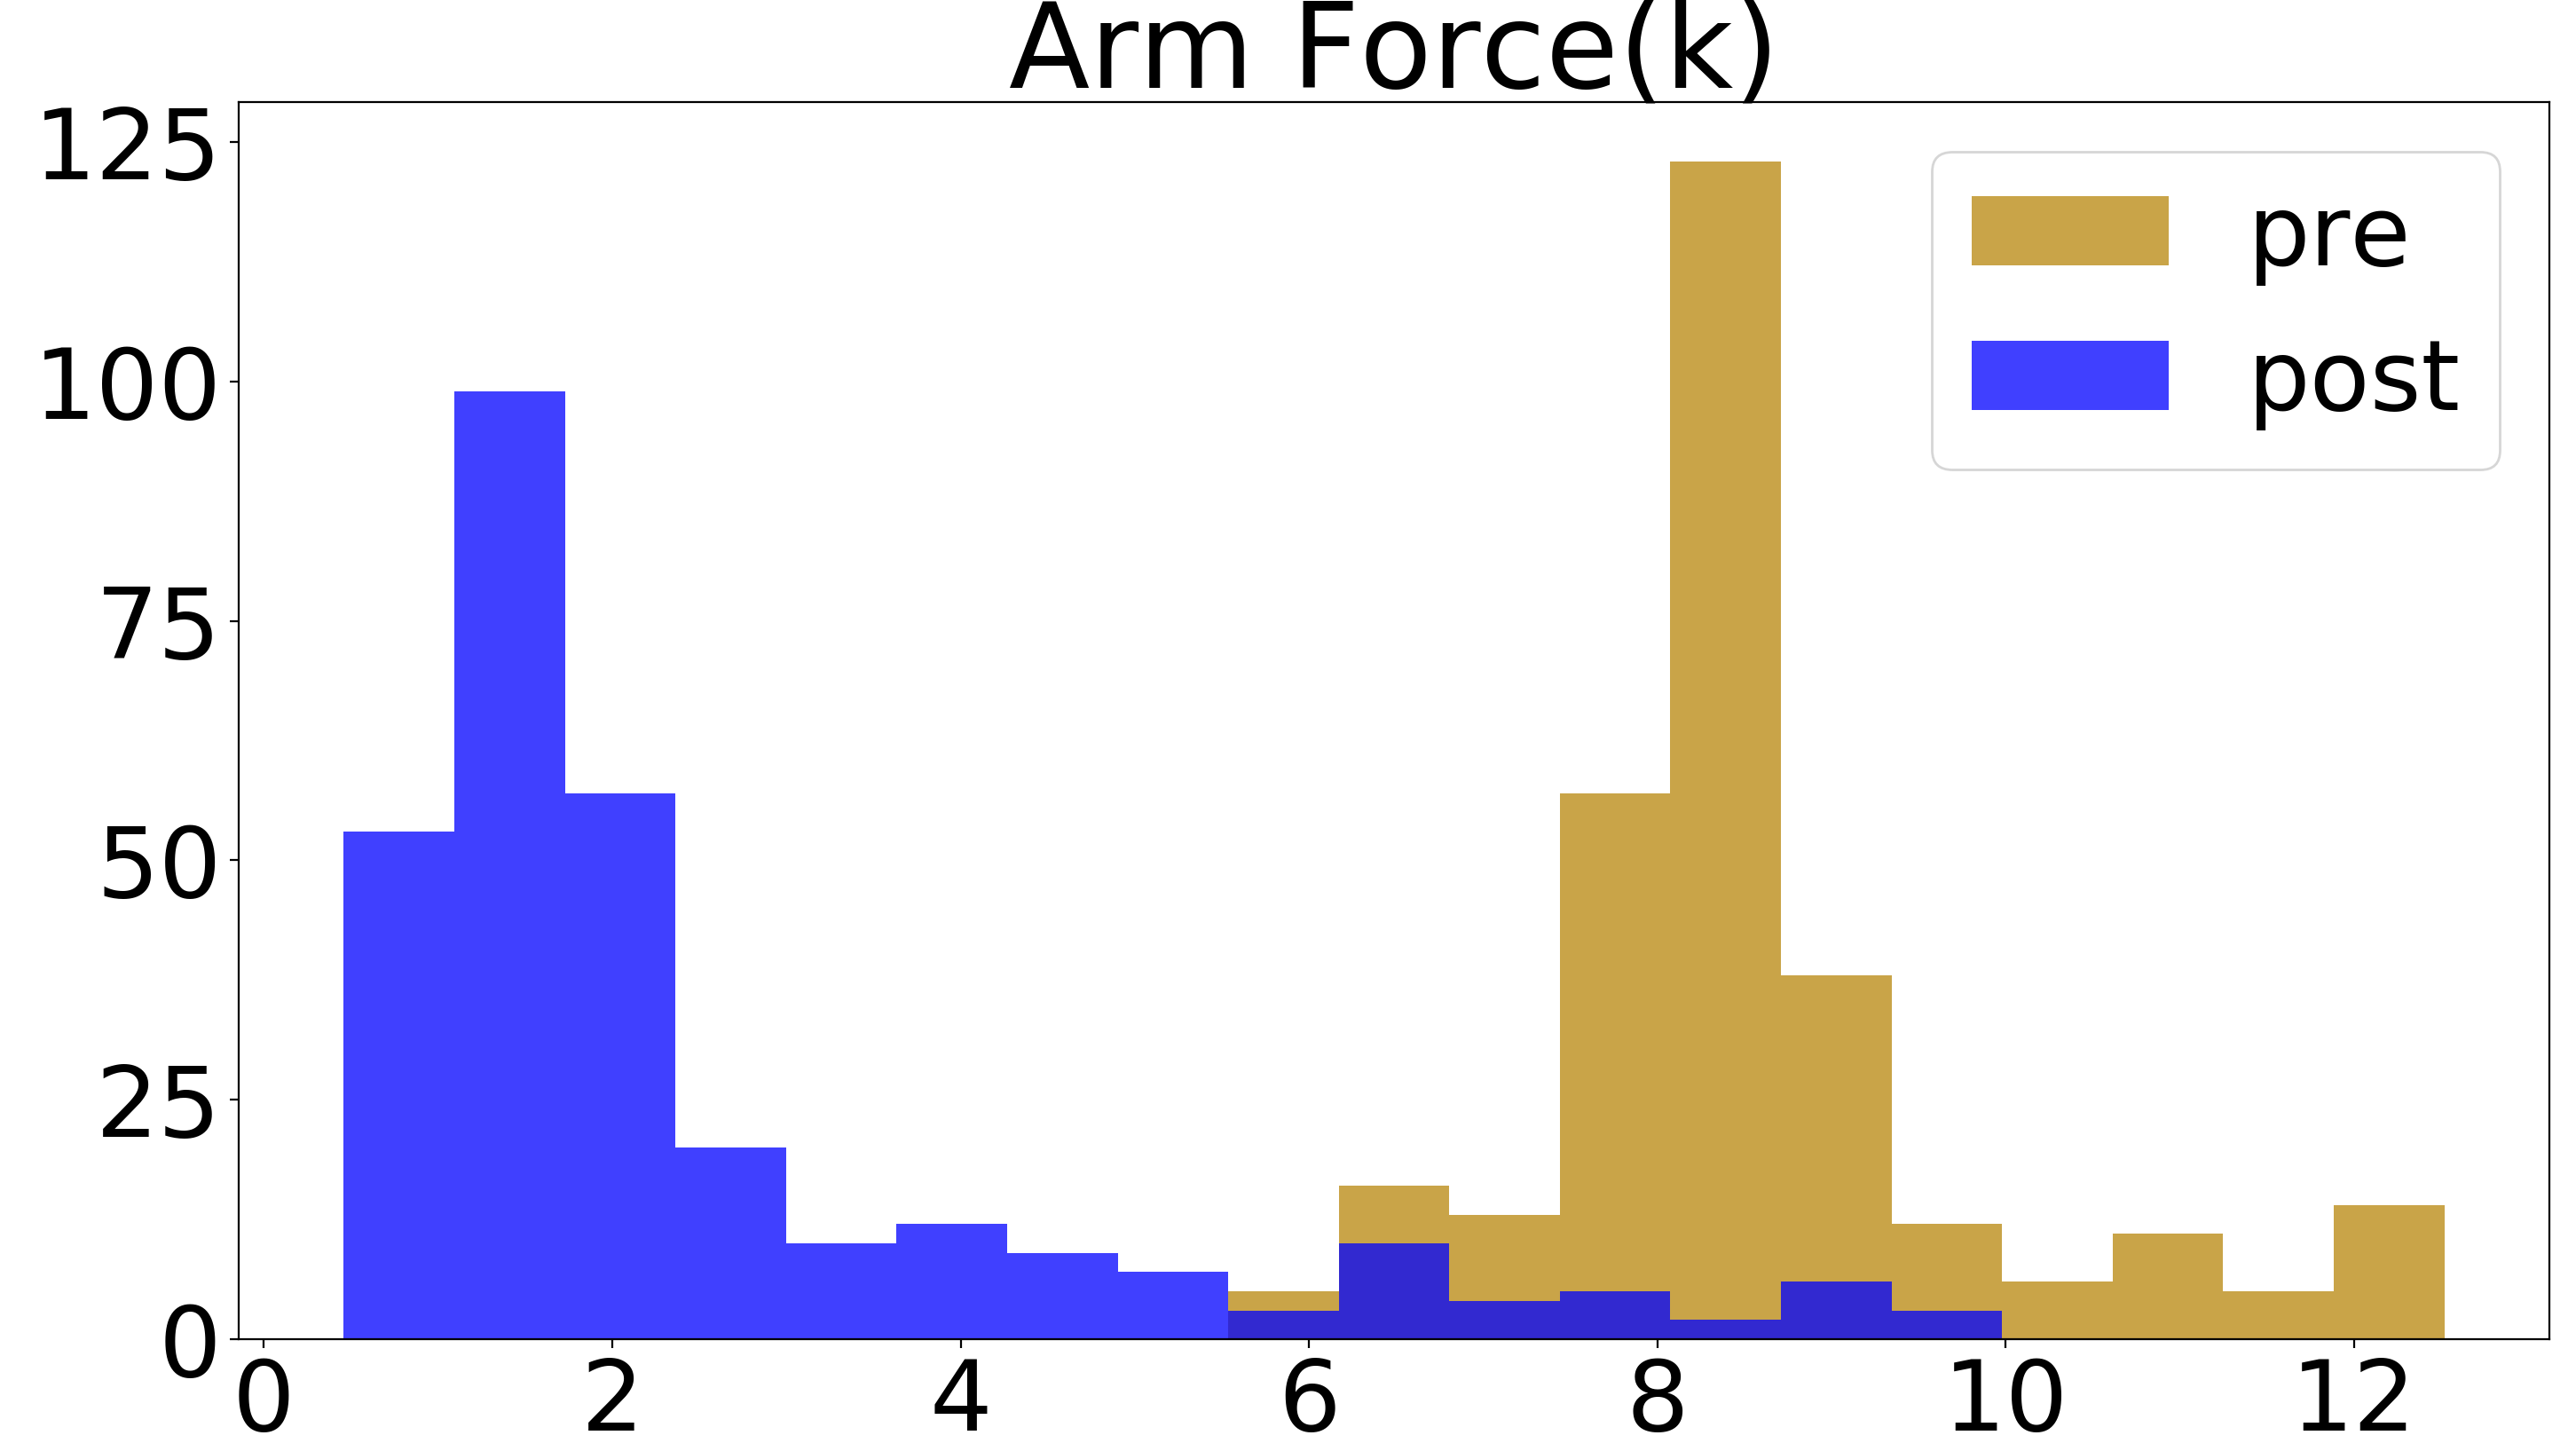
\includegraphics[width=0.3\textwidth]{pictures/hist_arm_task_k.png}
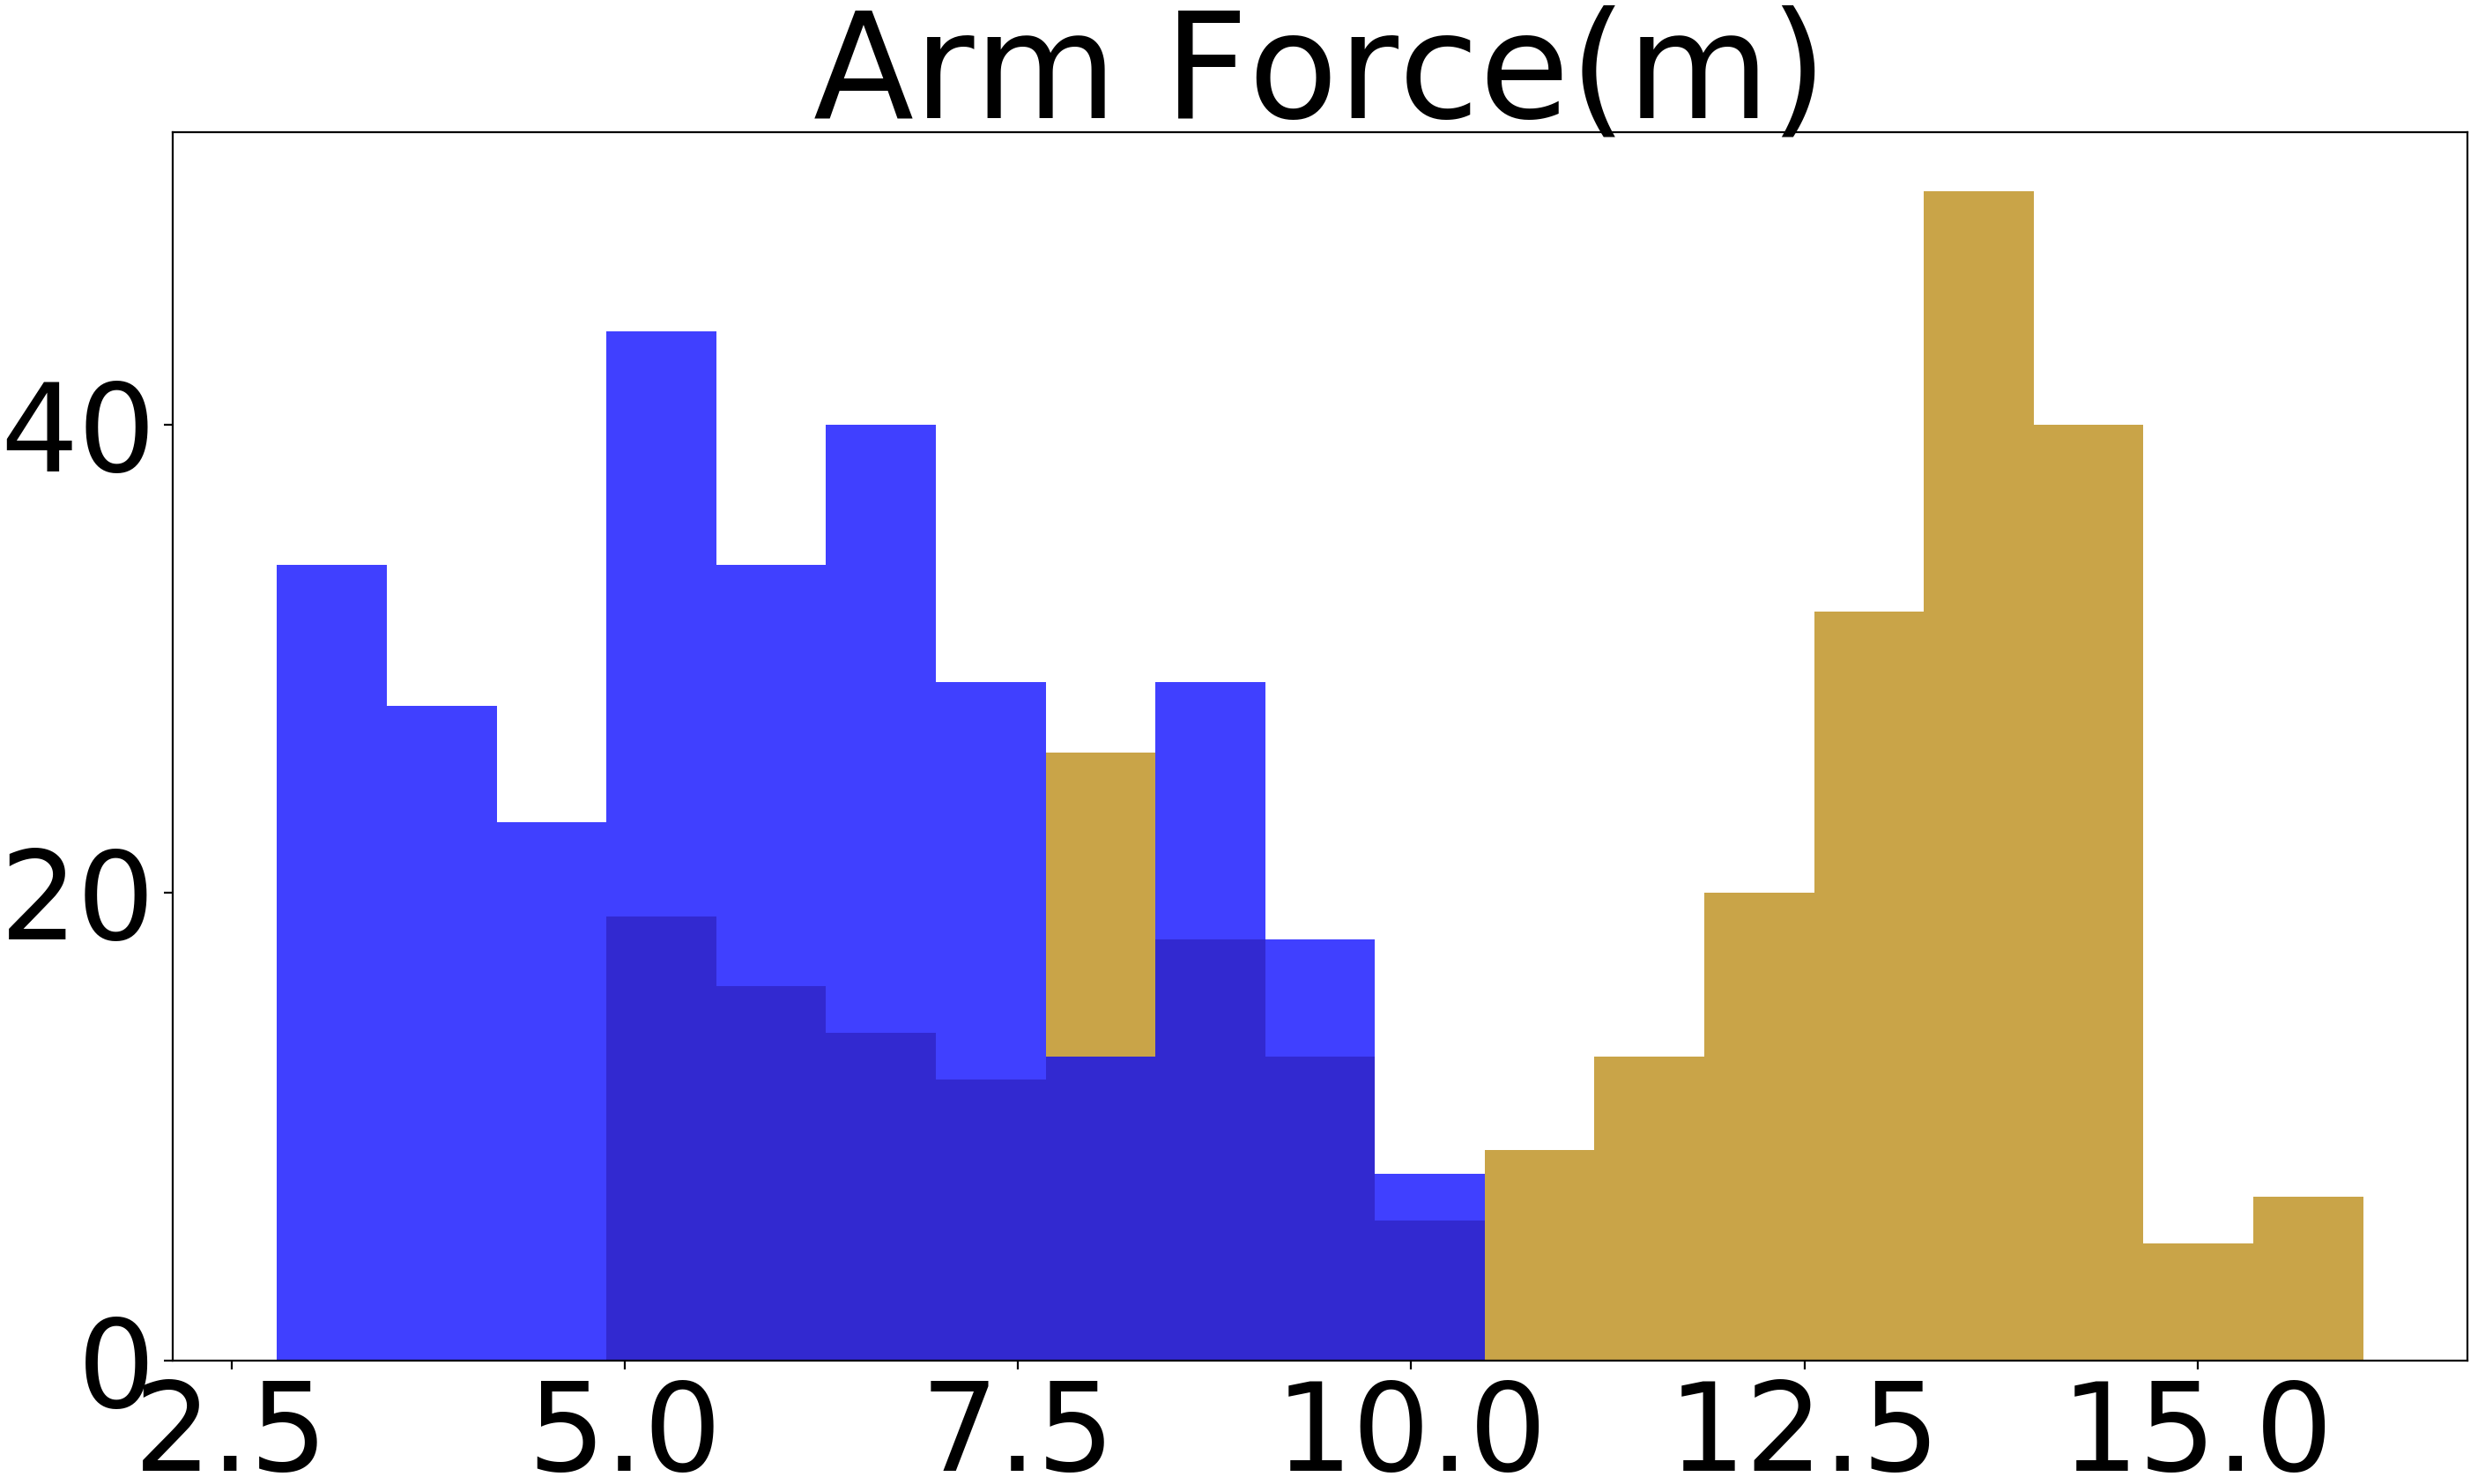
\includegraphics[width=0.3\textwidth]{pictures/hist_arm_task_m.png}
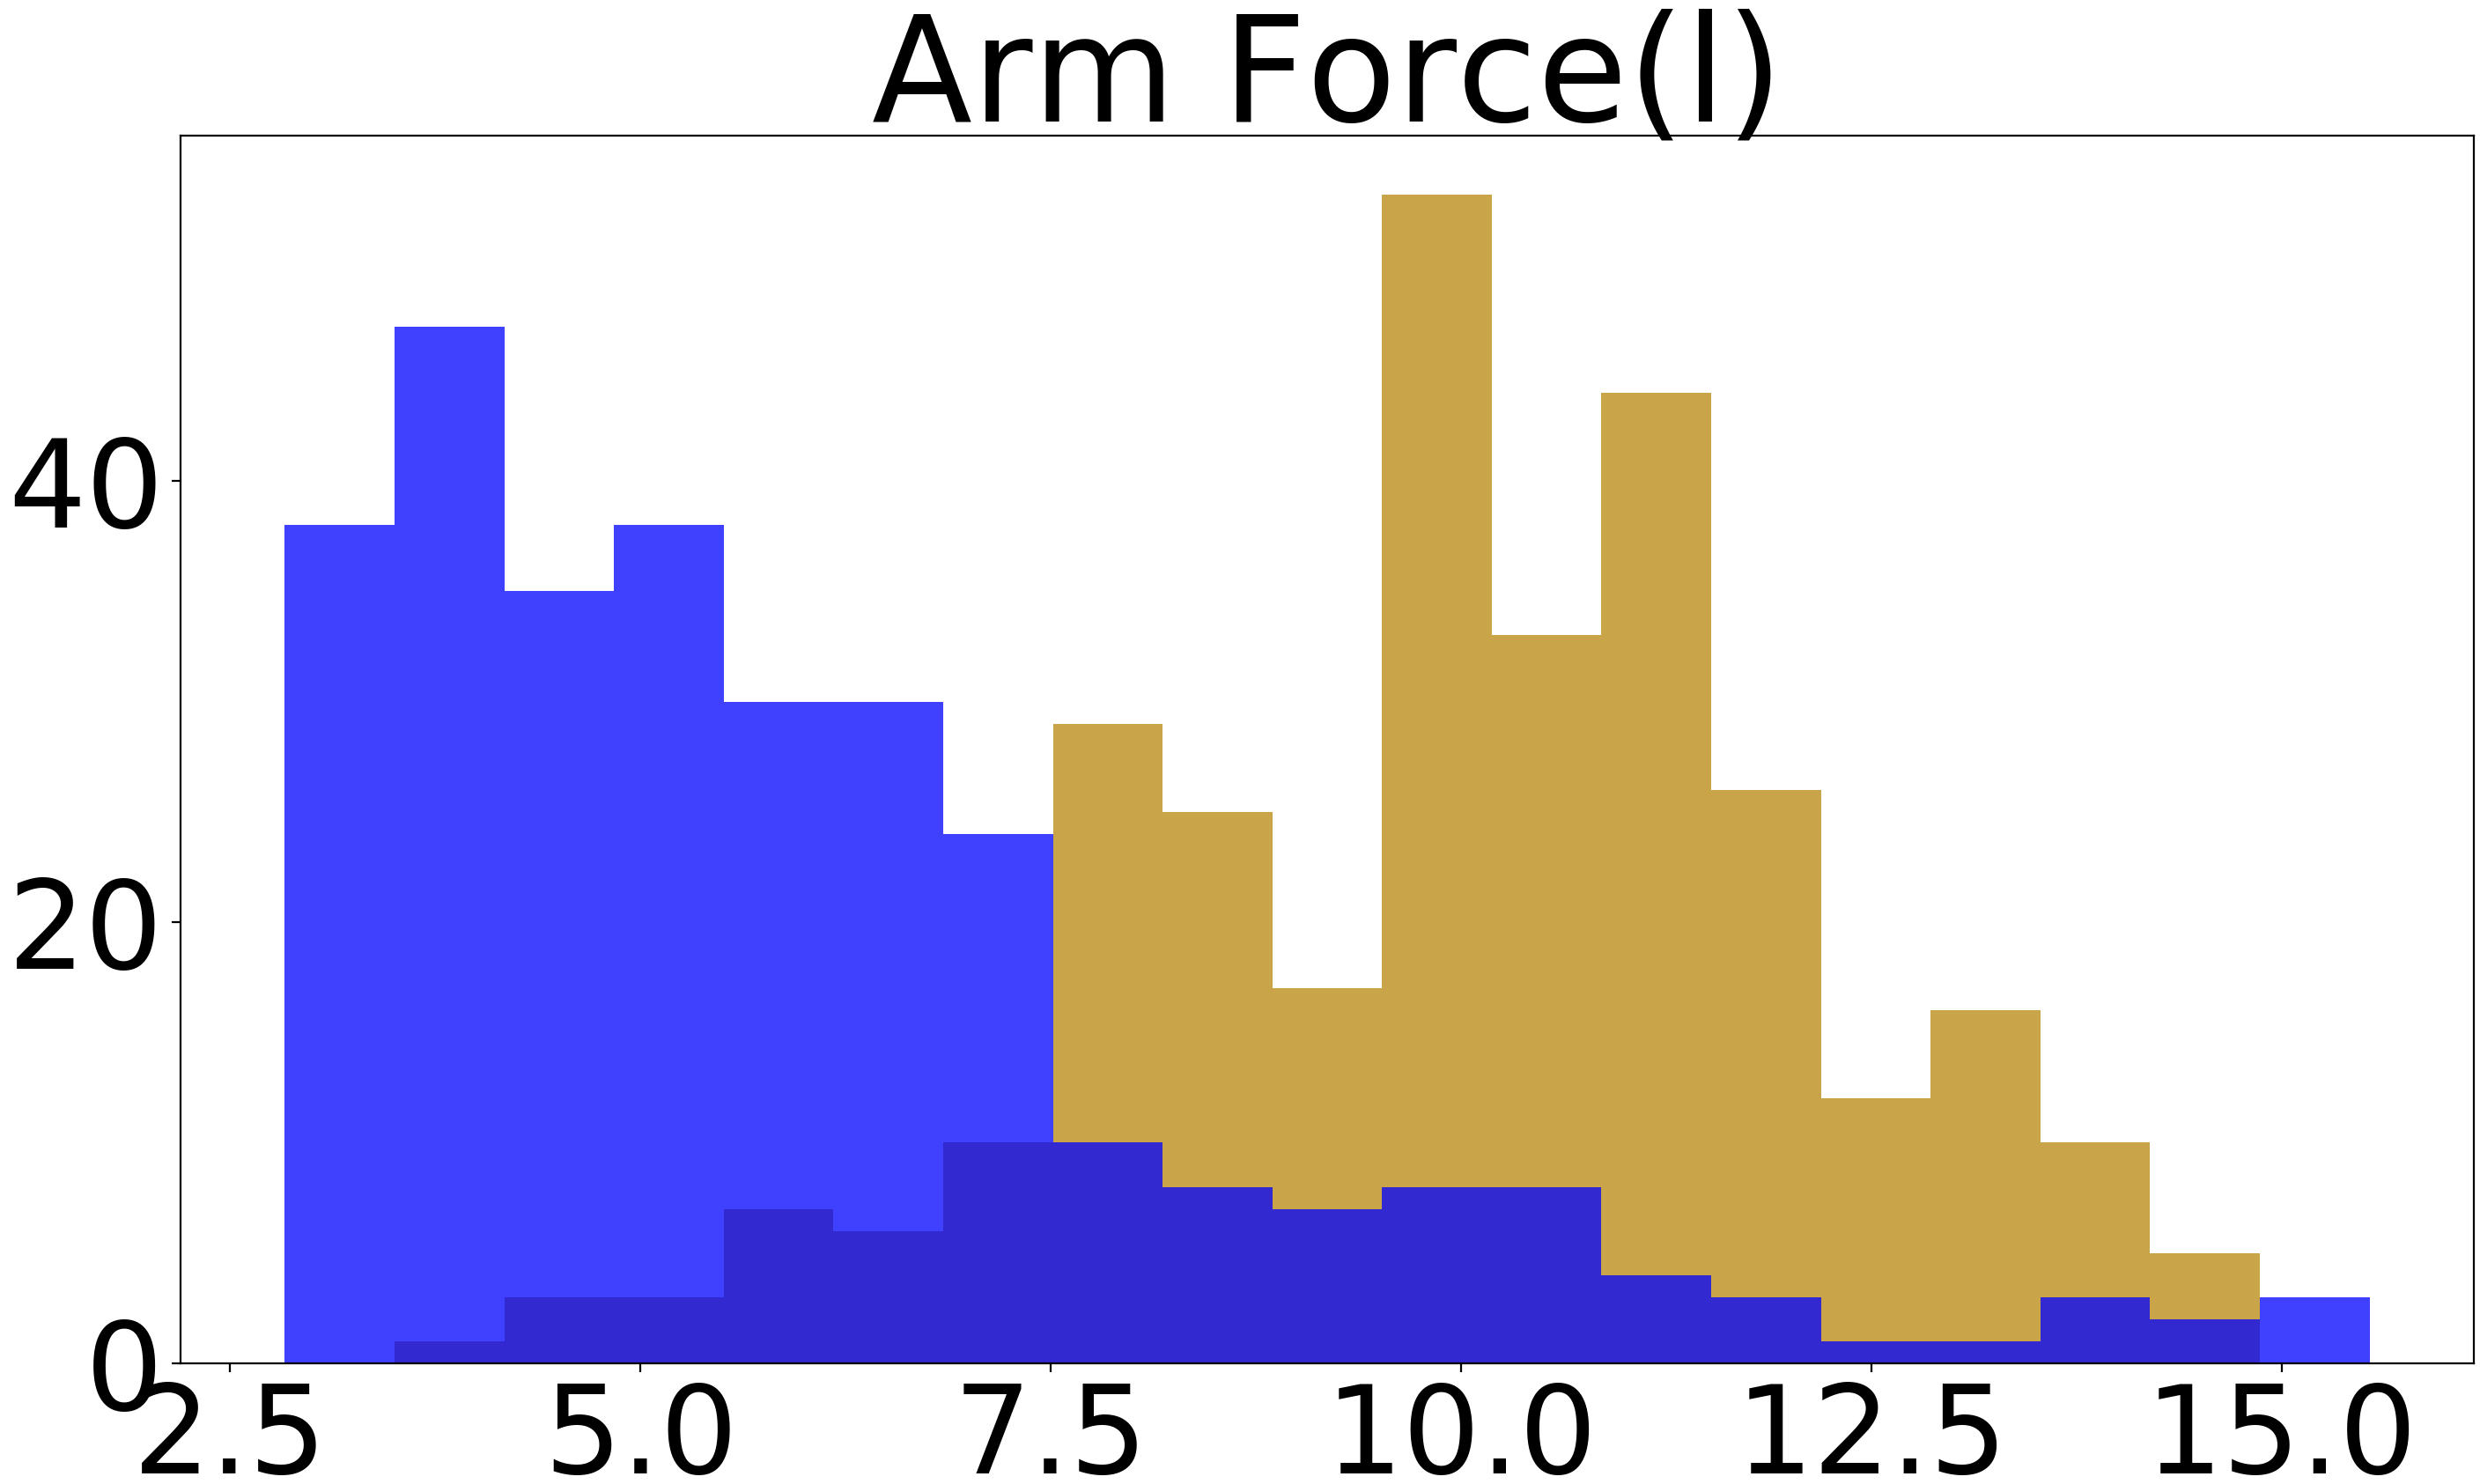
\includegraphics[width=0.3\textwidth]{pictures/hist_arm_task_l.png}
\\
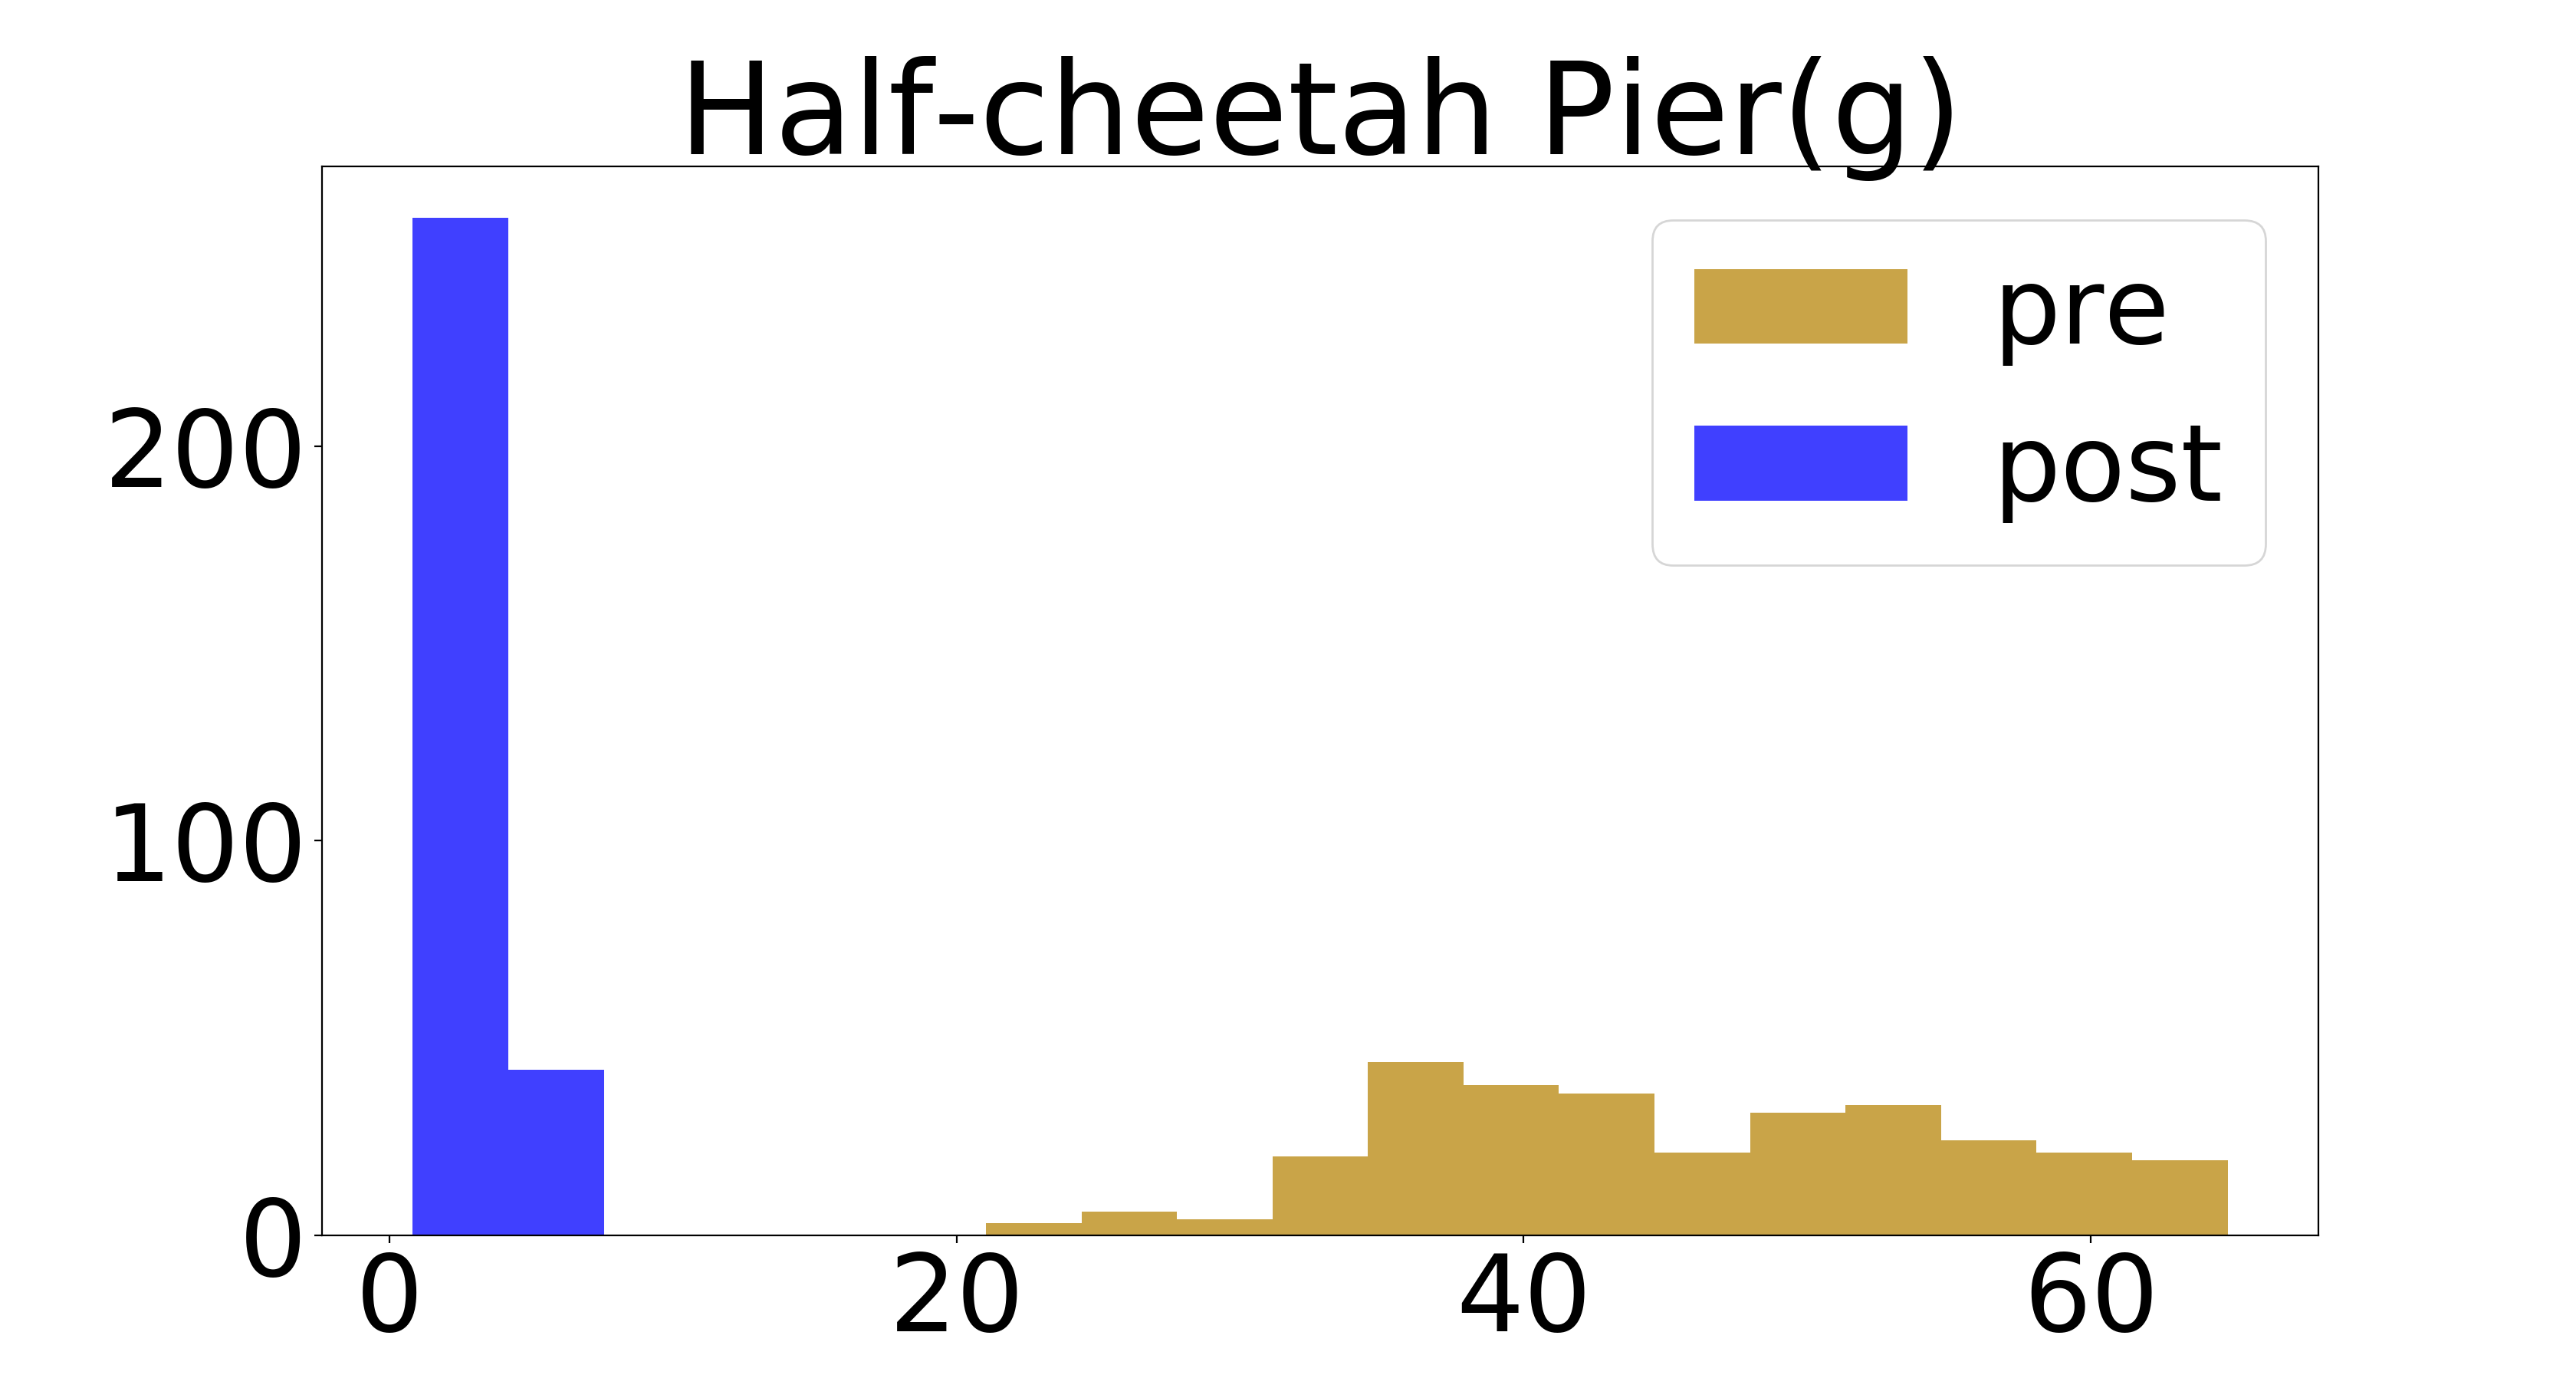
\includegraphics[width=0.3\textwidth]{pictures/hist_hc_pier.png}
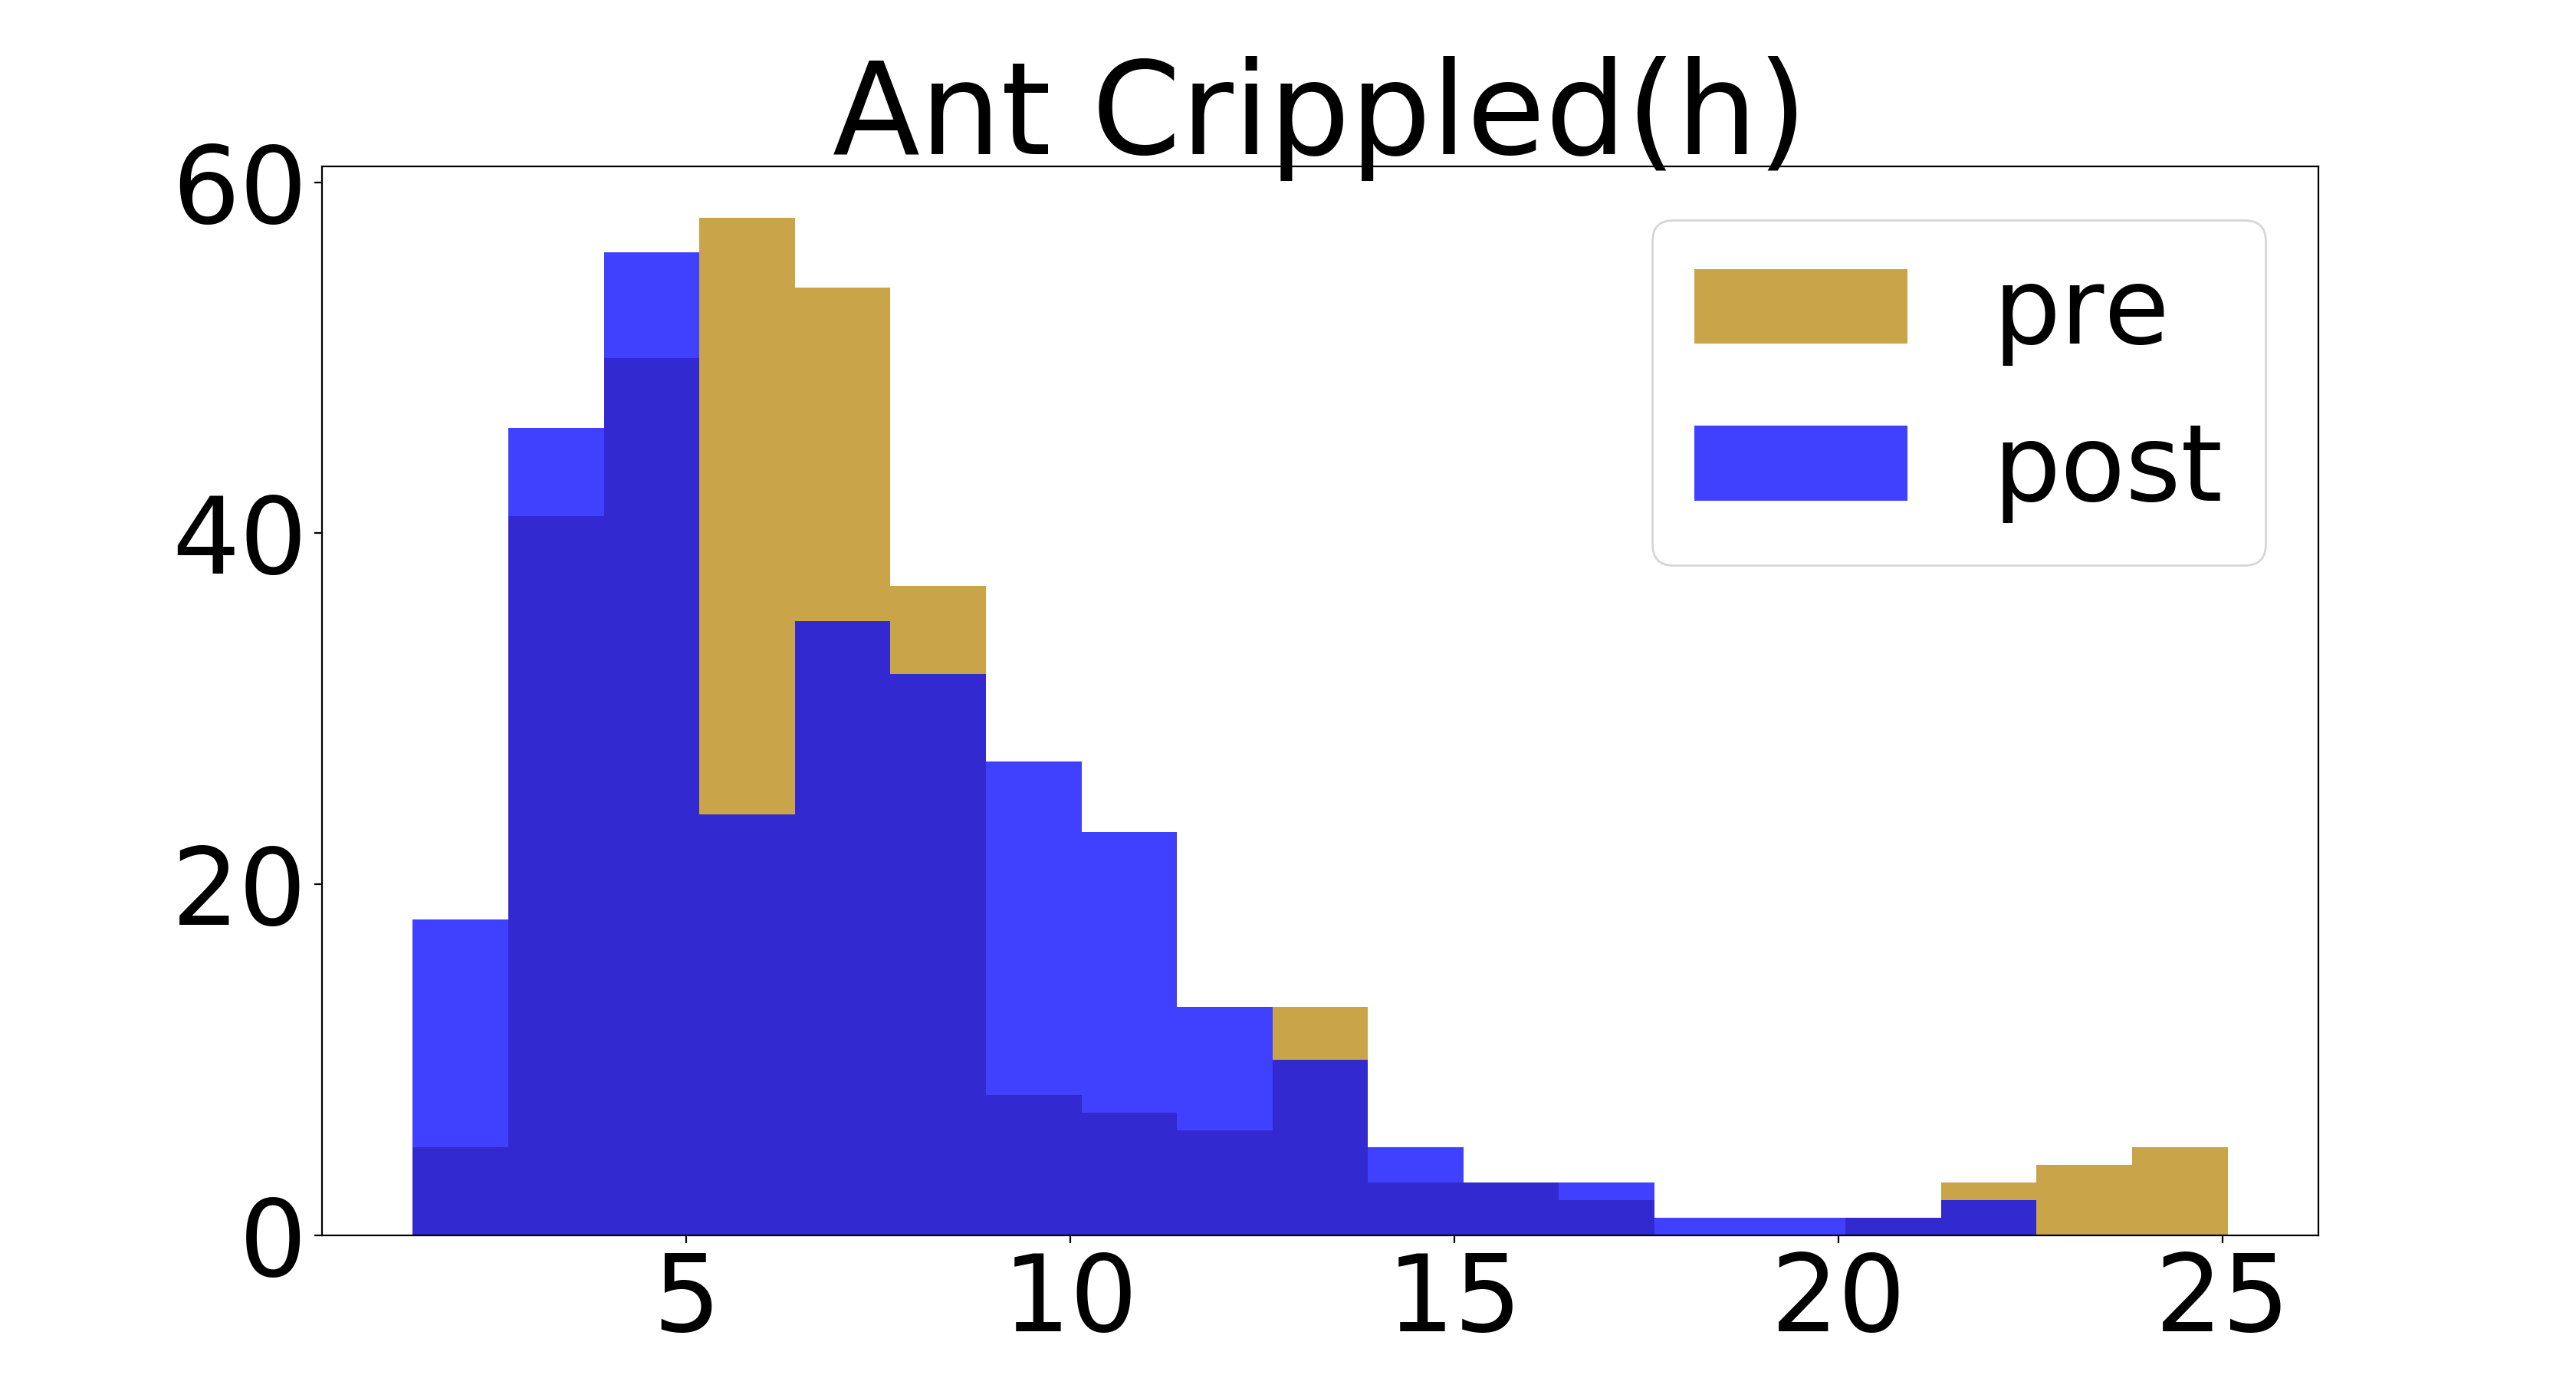
\includegraphics[width=0.3\textwidth]{pictures/hist_ant_task_h.png}
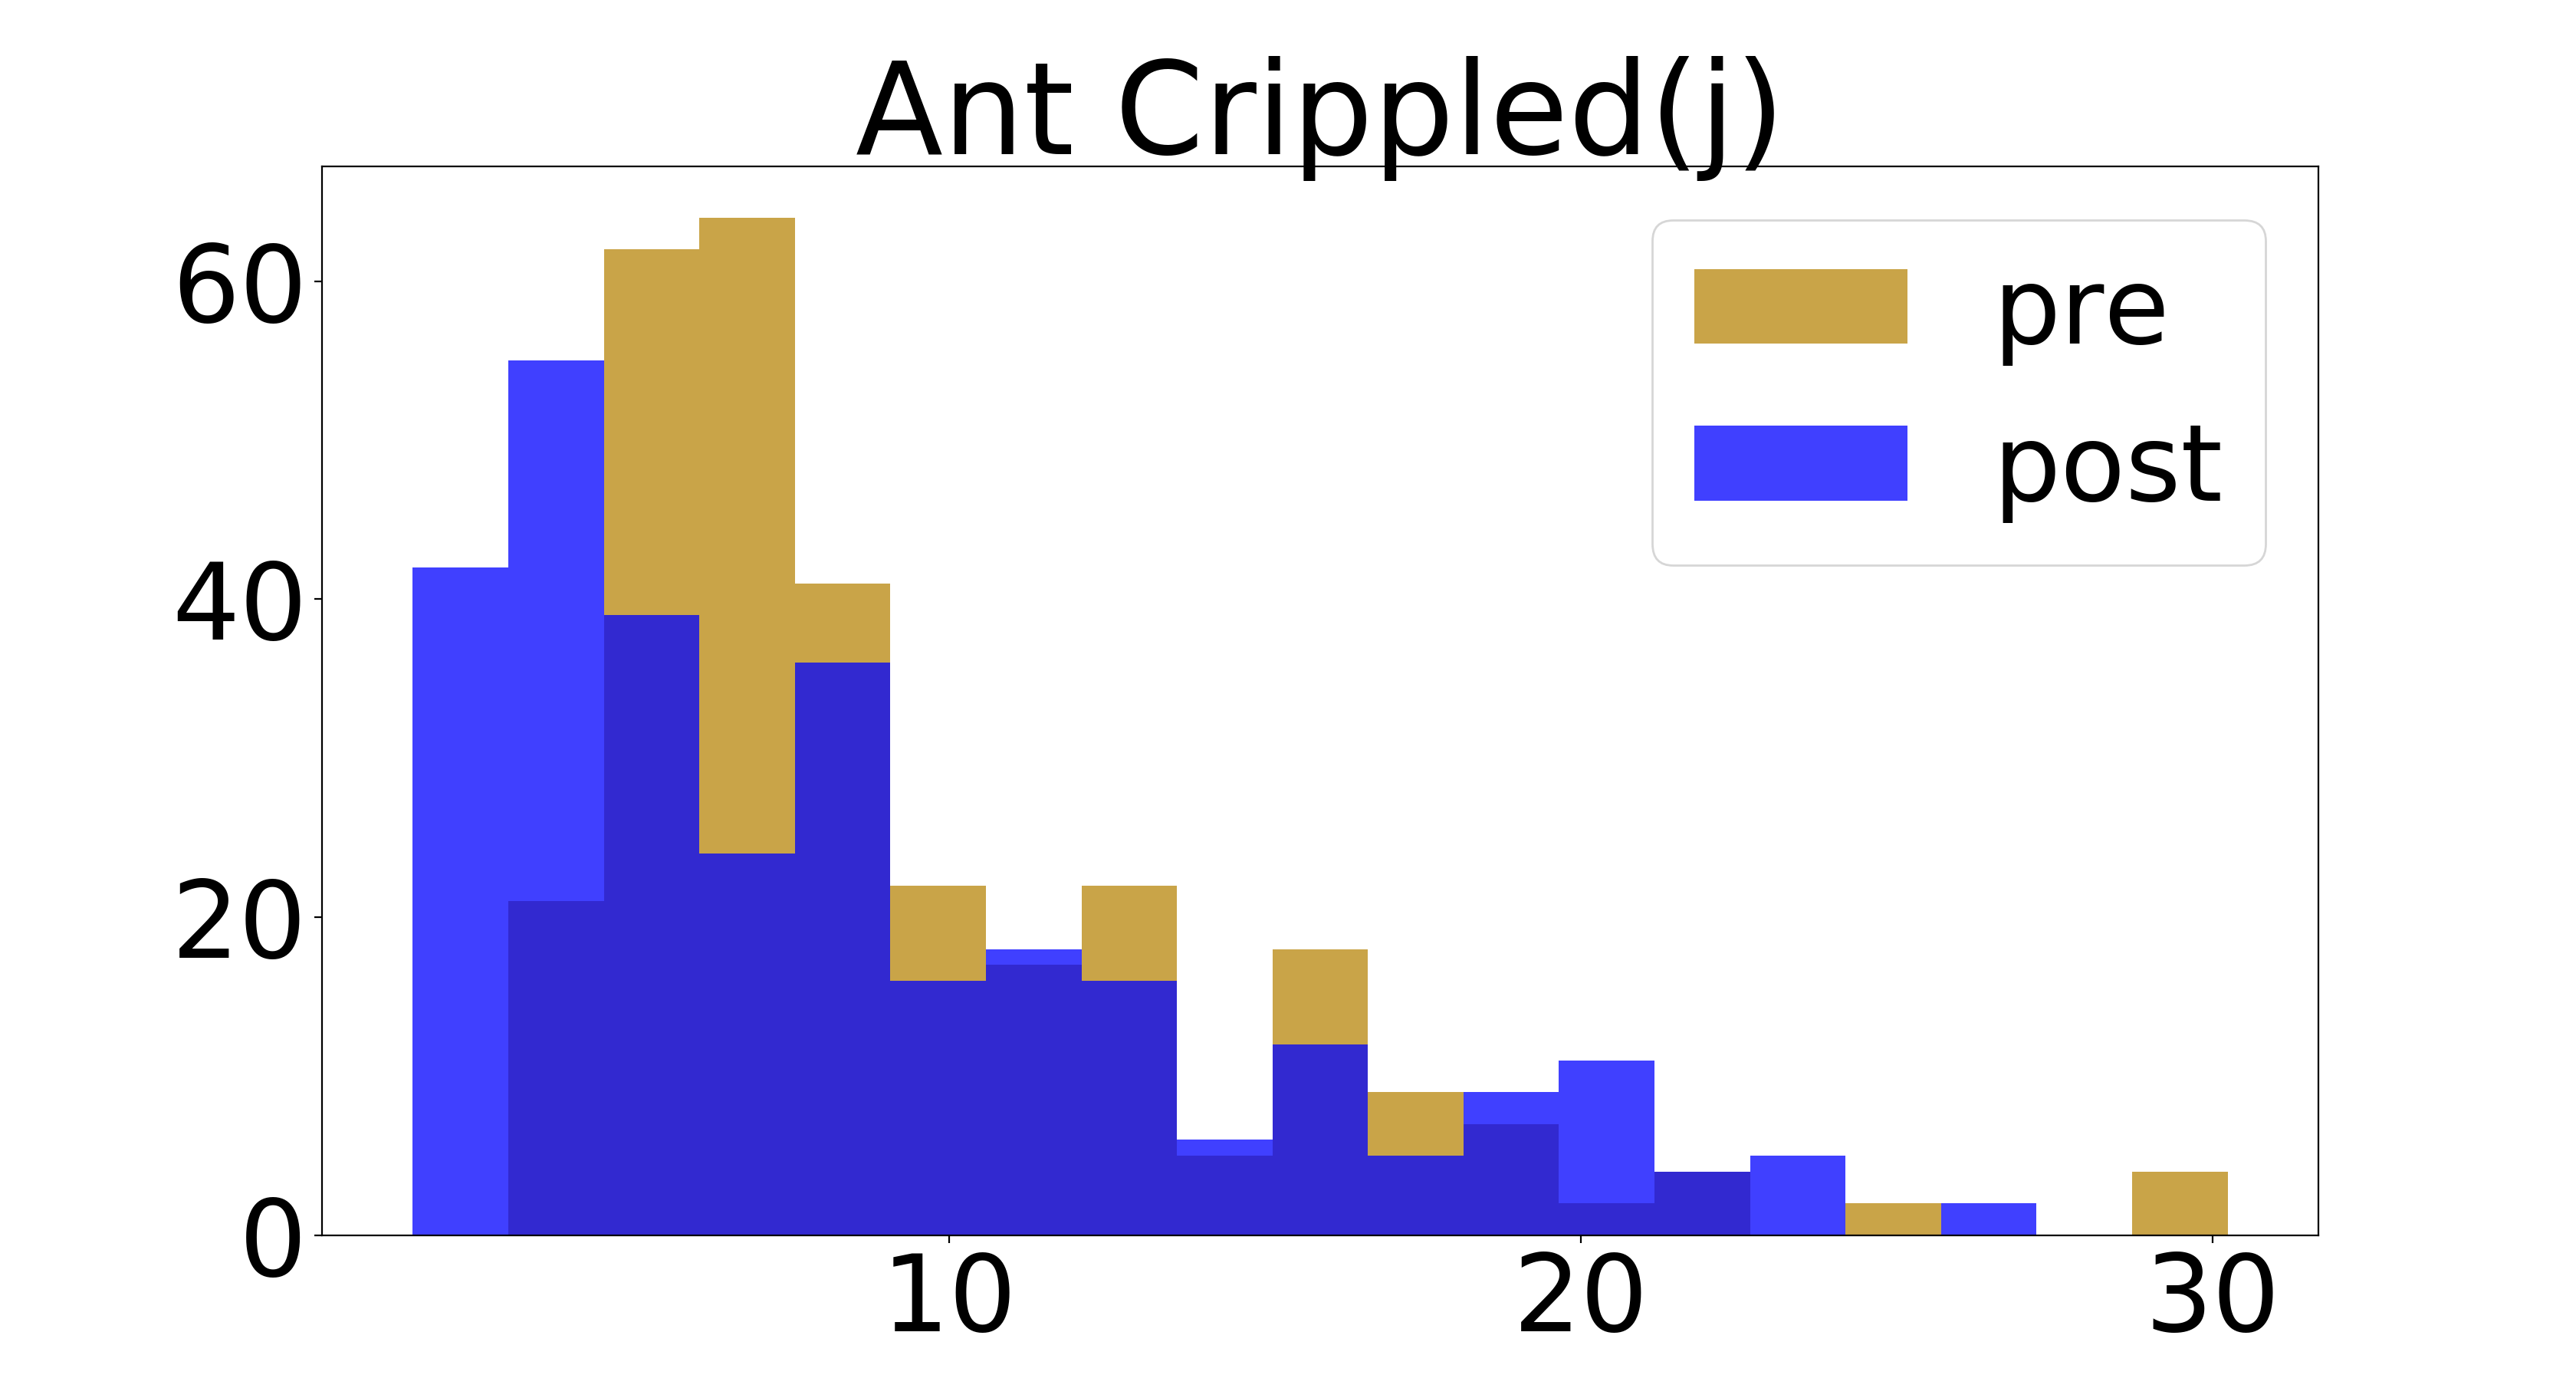
\includegraphics[width=0.3\textwidth]{pictures/hist_ant_task_j.png}
\\
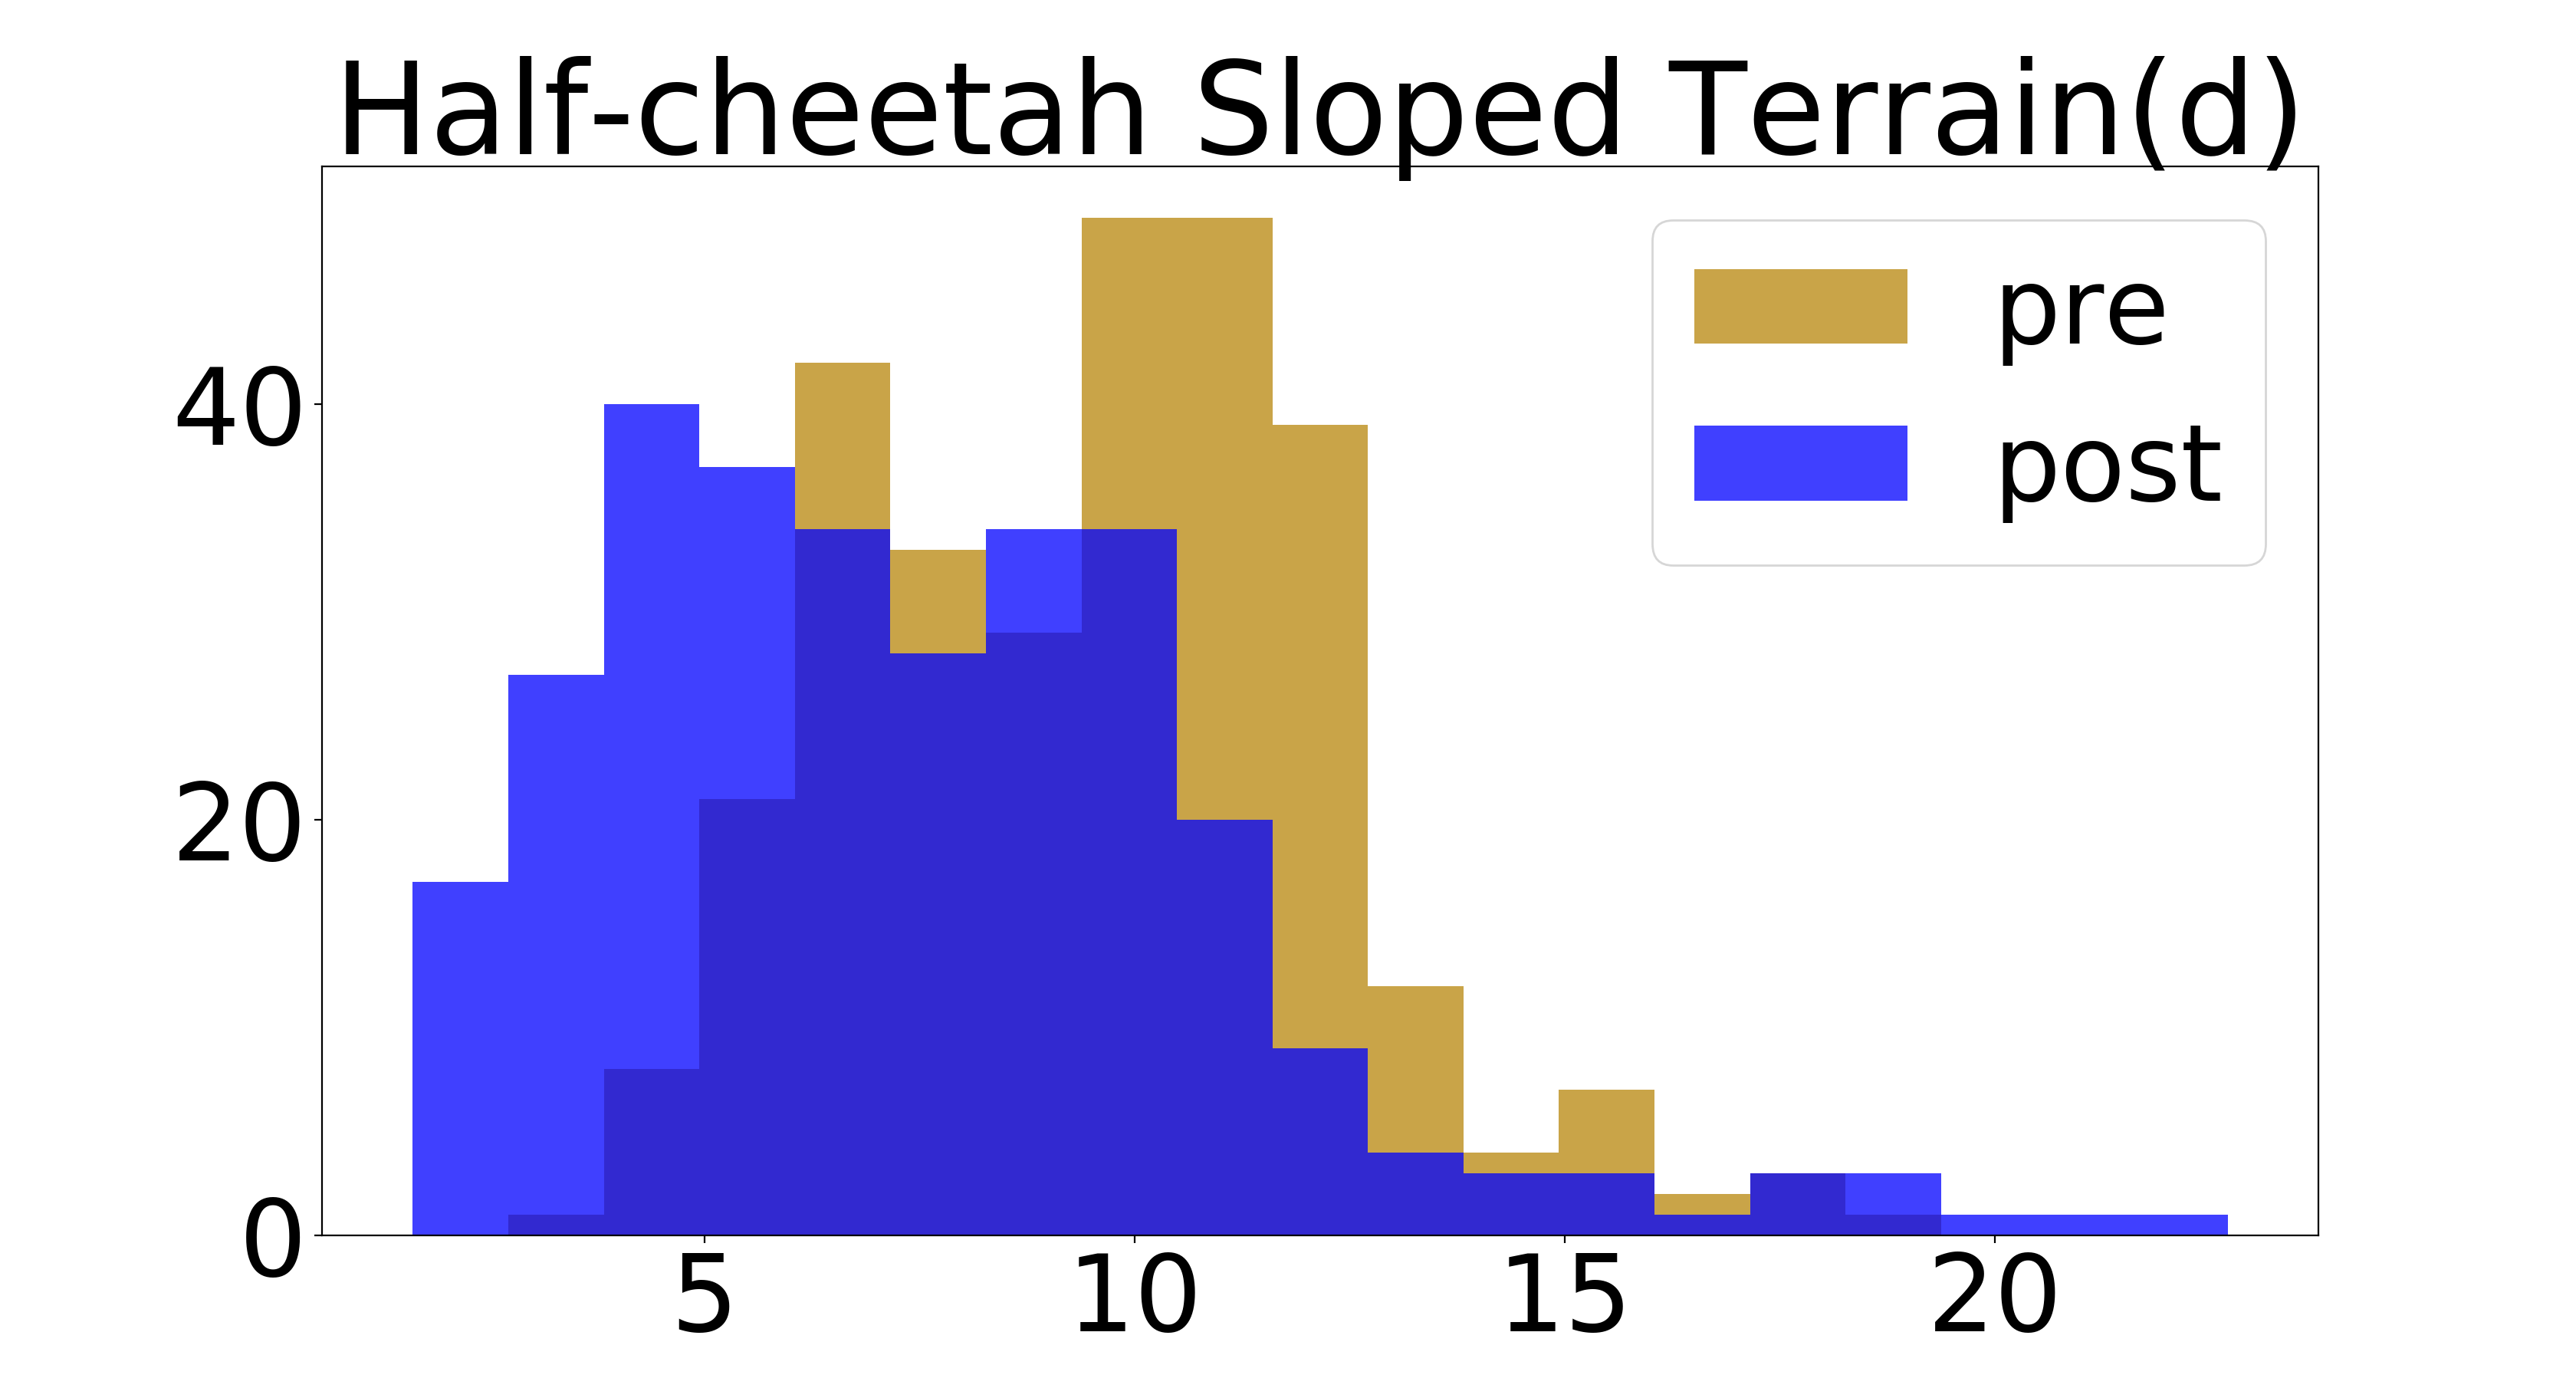
\includegraphics[width=0.3\textwidth]{pictures/hist_hc_gentle.png}
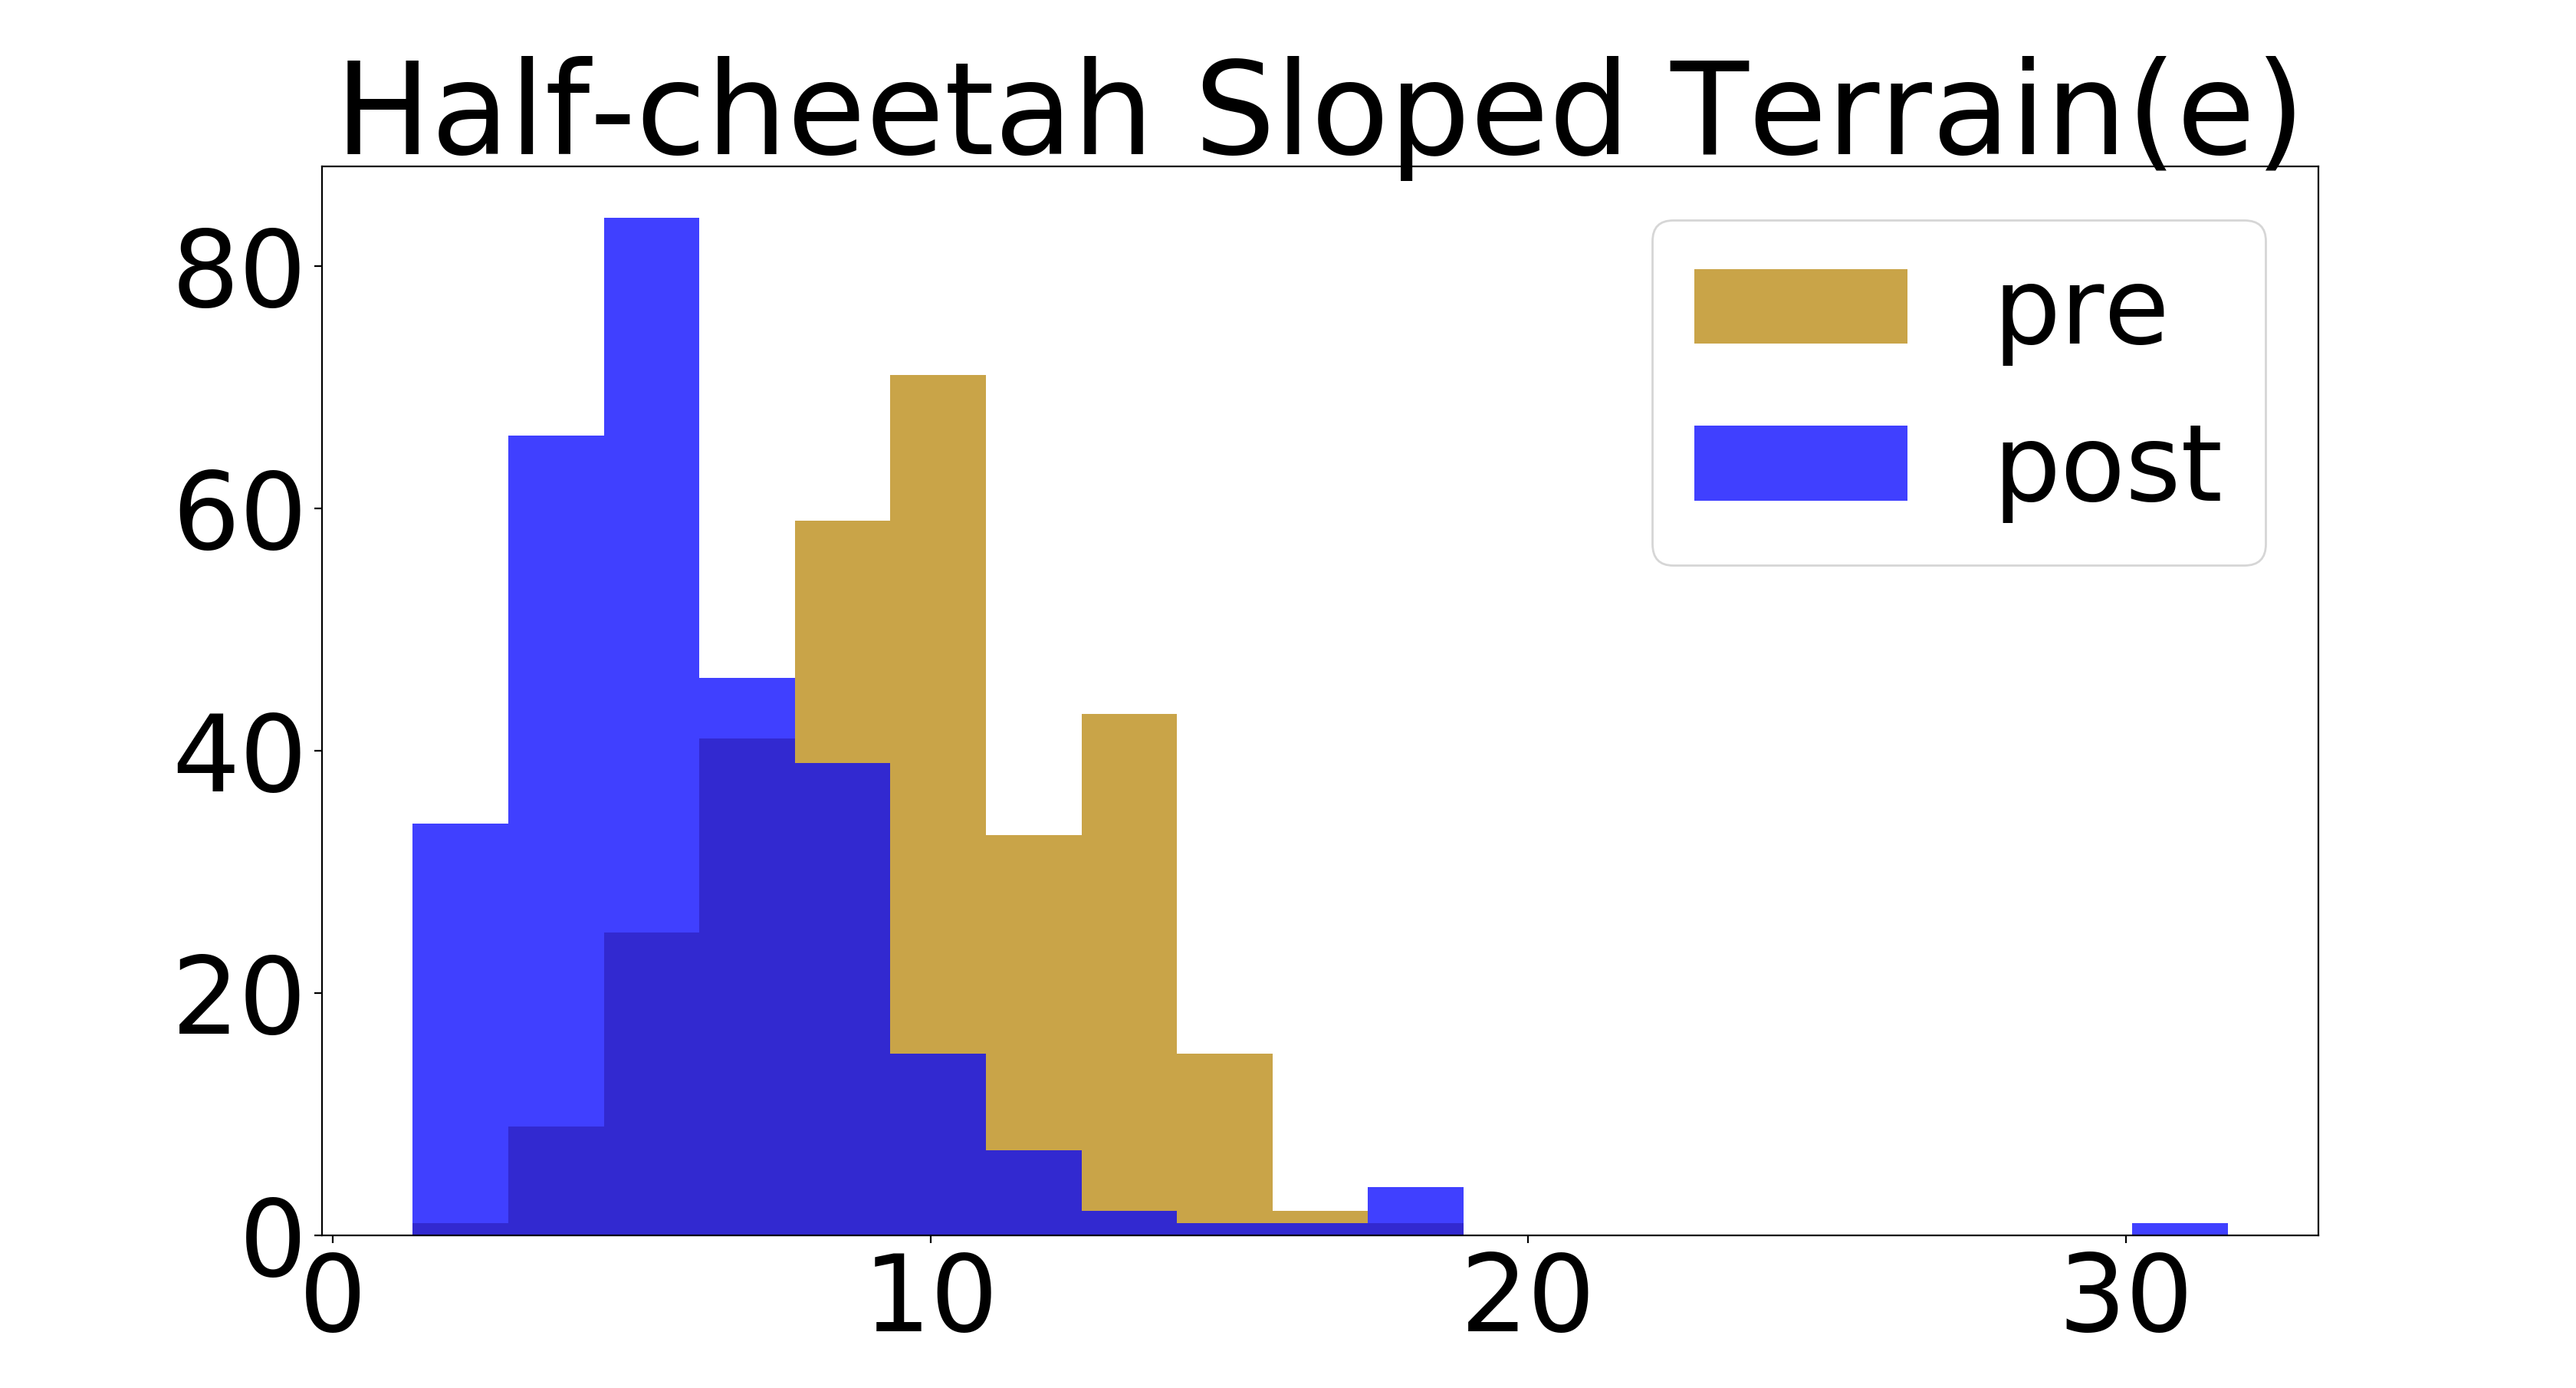
\includegraphics[width=0.3\textwidth]{pictures/hist_hc_hill.png}
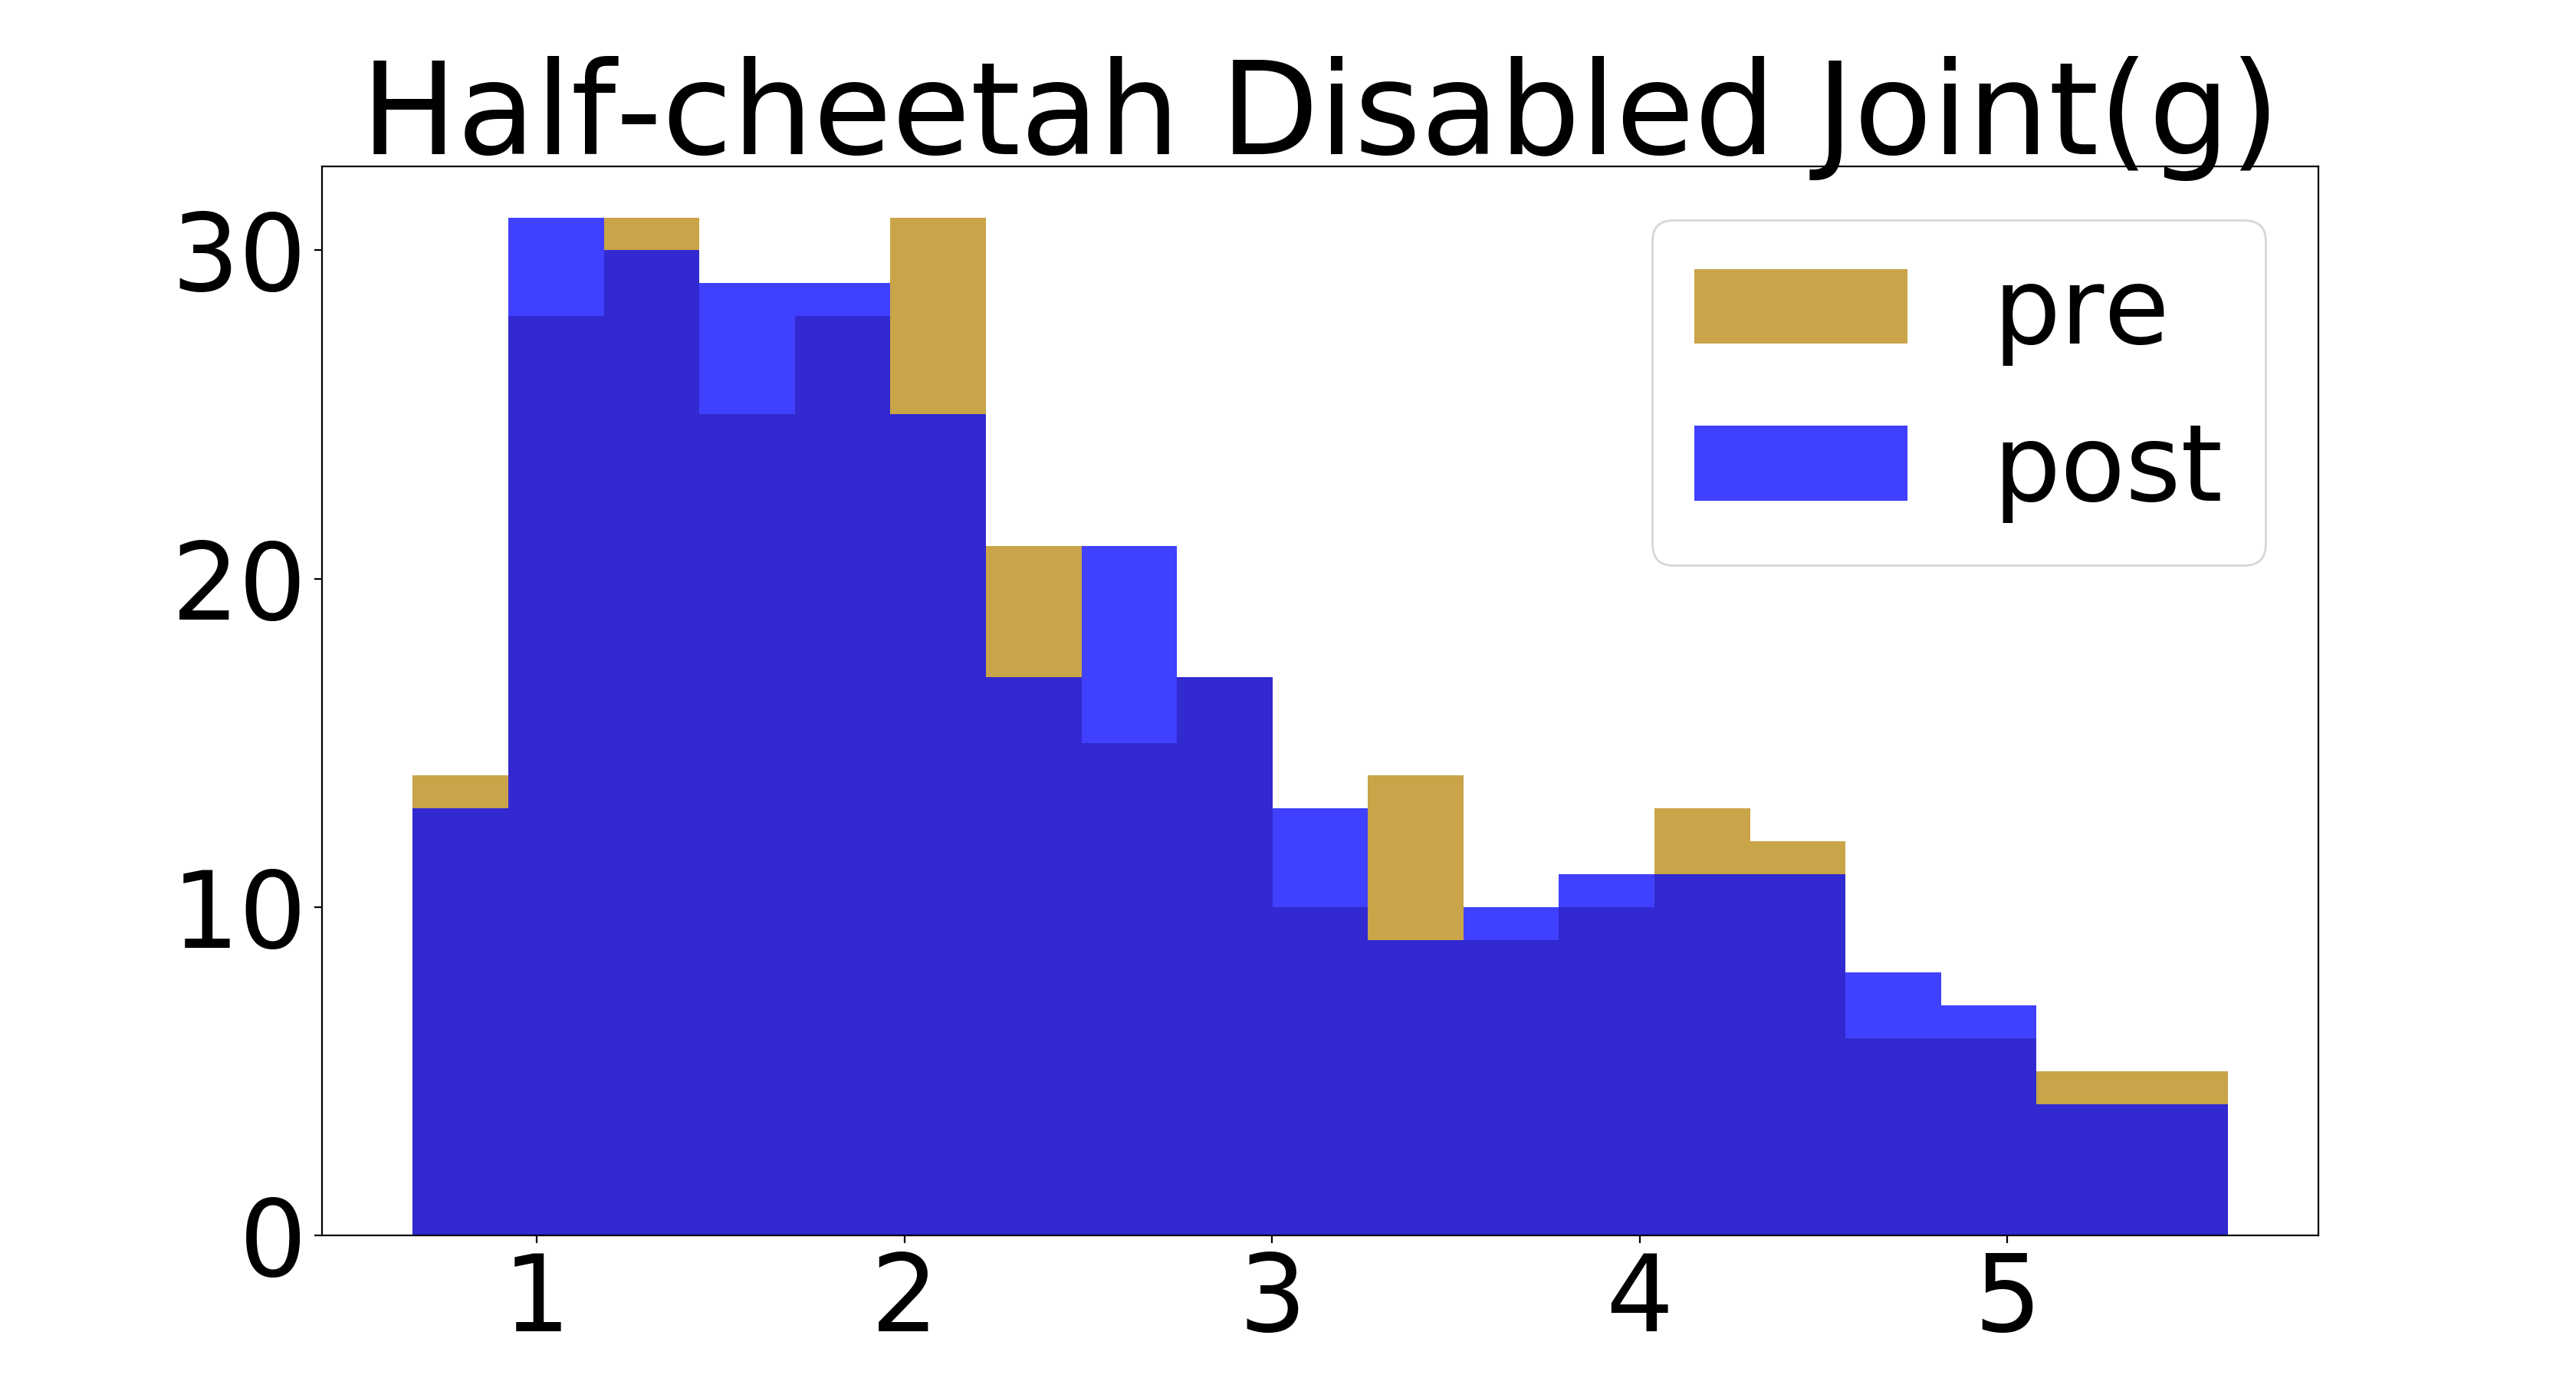
\includegraphics[width=0.3\textwidth]{pictures/hist_hc_disabled.png}
% \vspace{-0.8cm}
% \vspace{-0.1in}
\caption{\small Histogram of the $K$ step normalized error across different tasks. GrBAL accomplishes lower model error when using the parameters given by the update rule. }
\label{fig:hist}
% \vspace{-0.1in}
\end{figure}
\begin{figure}[H]
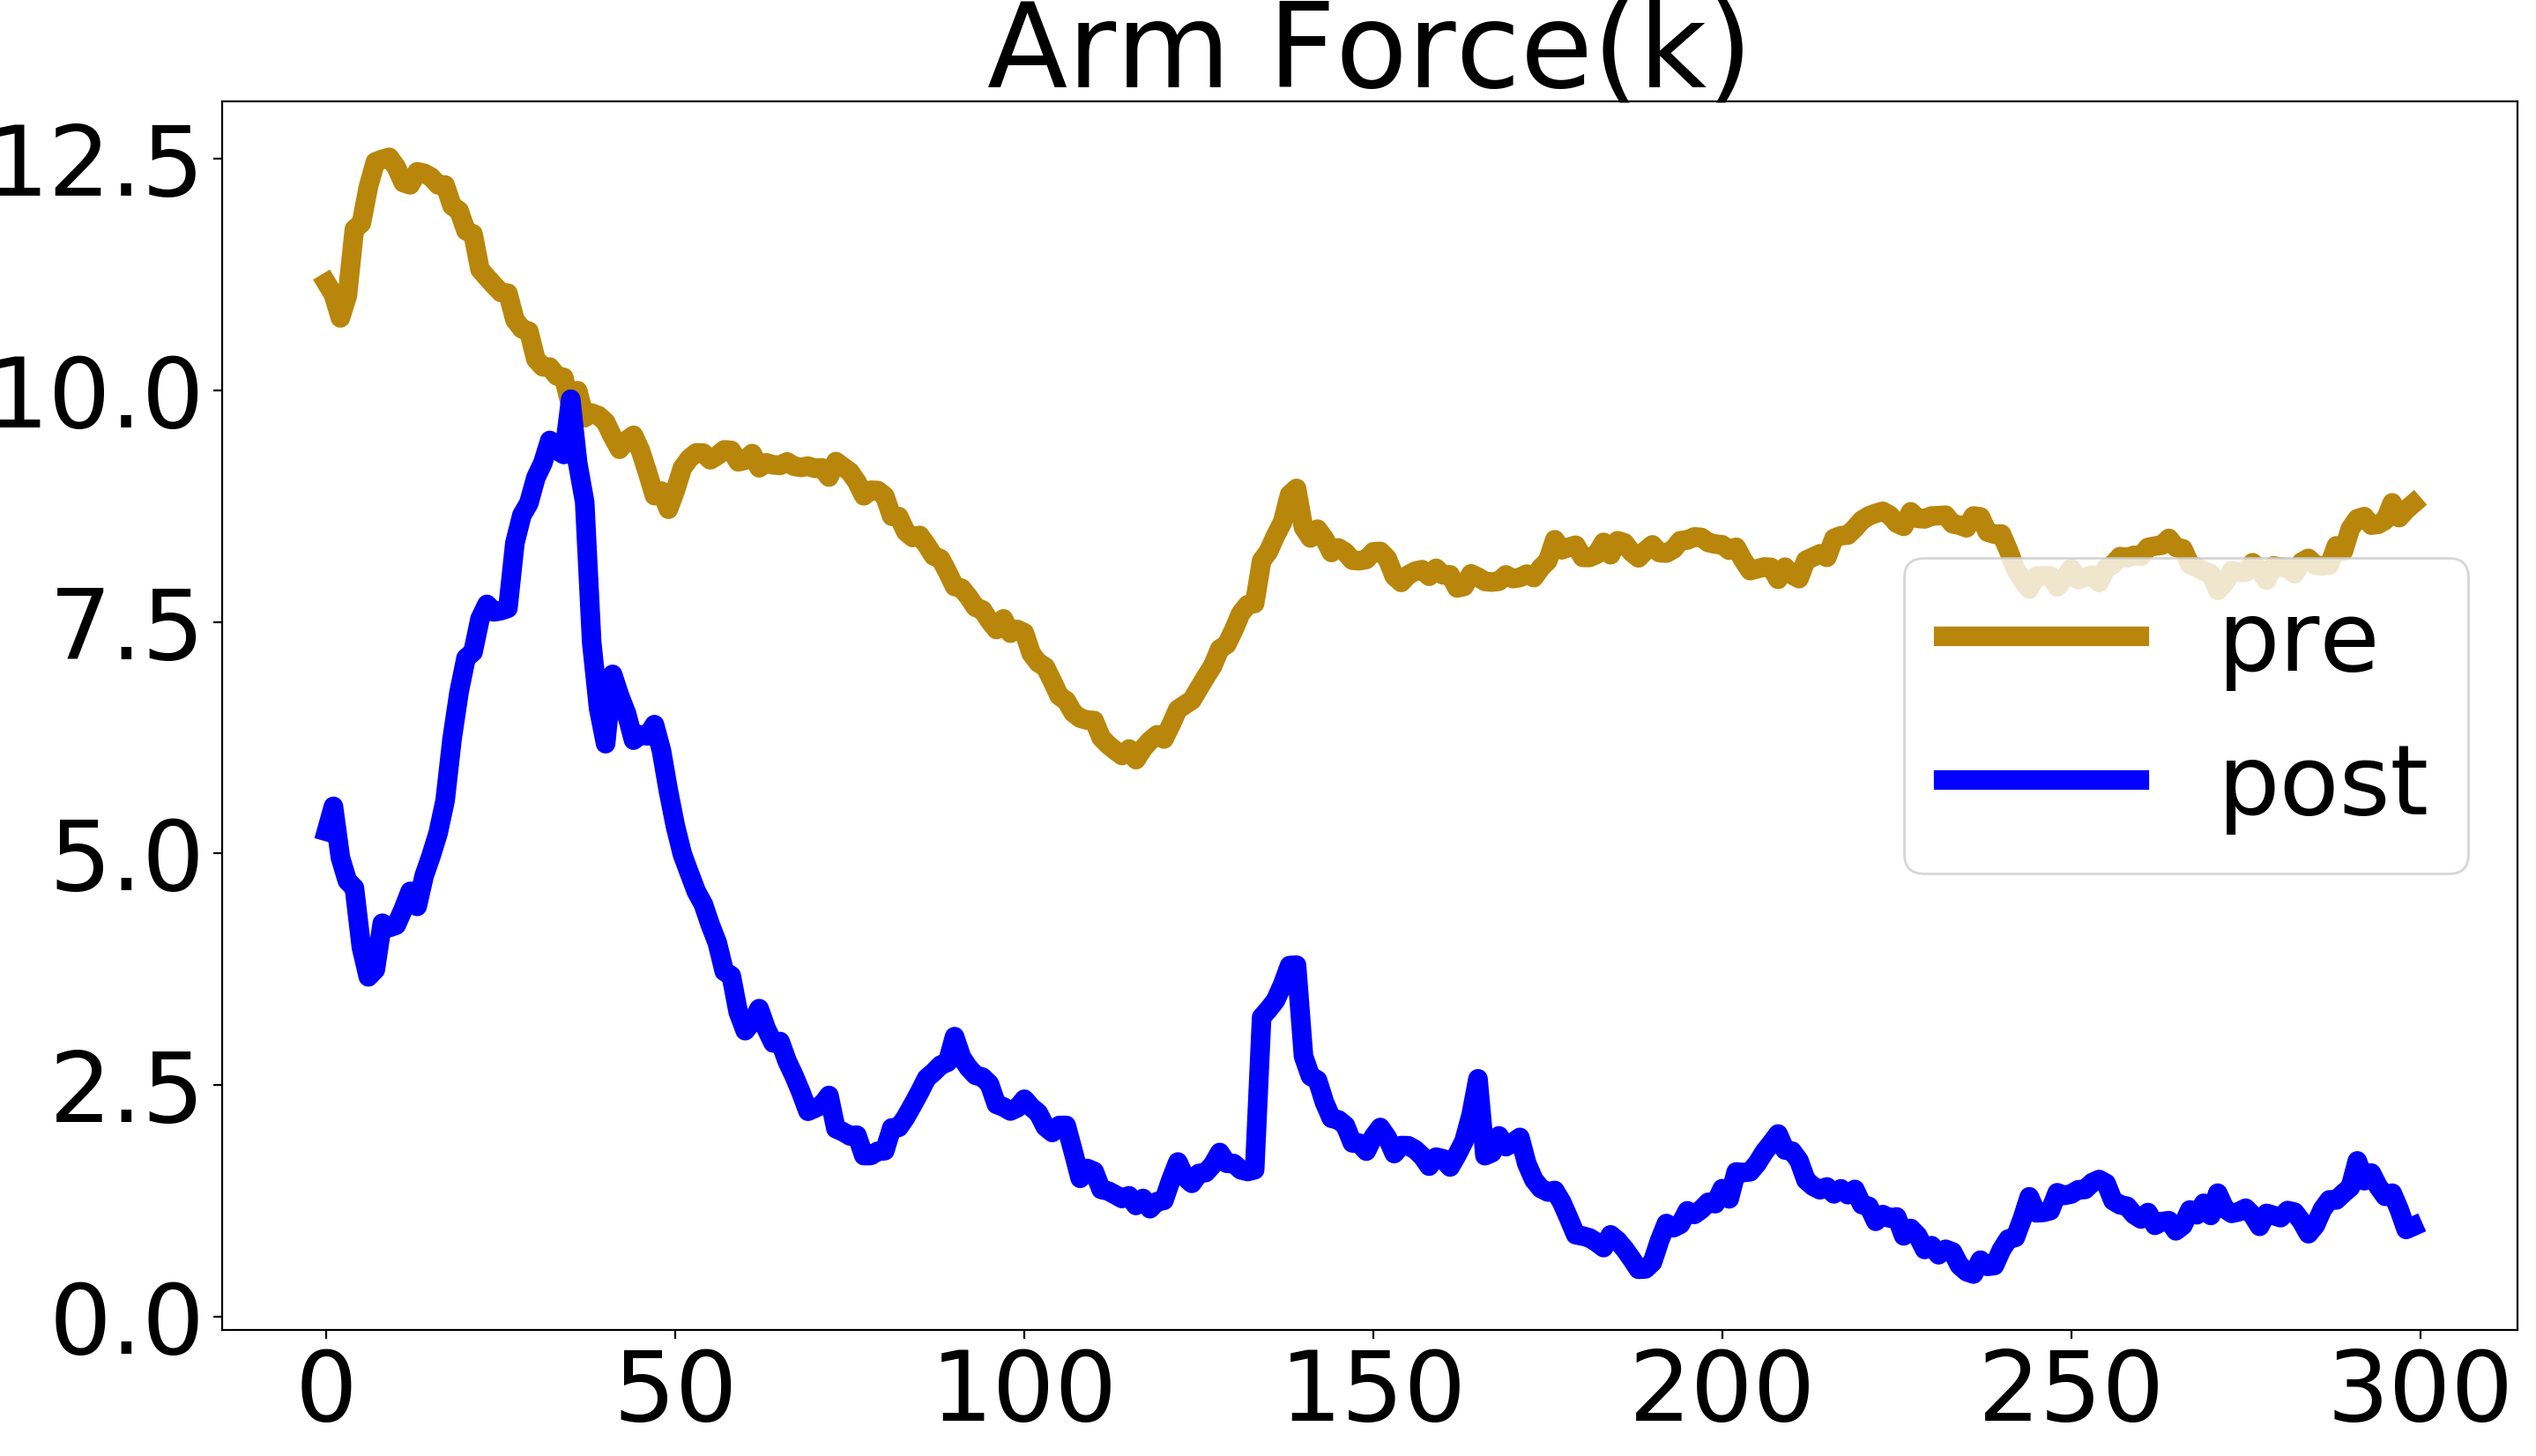
\includegraphics[width=0.3\textwidth]{pictures/error_arm_task_k.png}
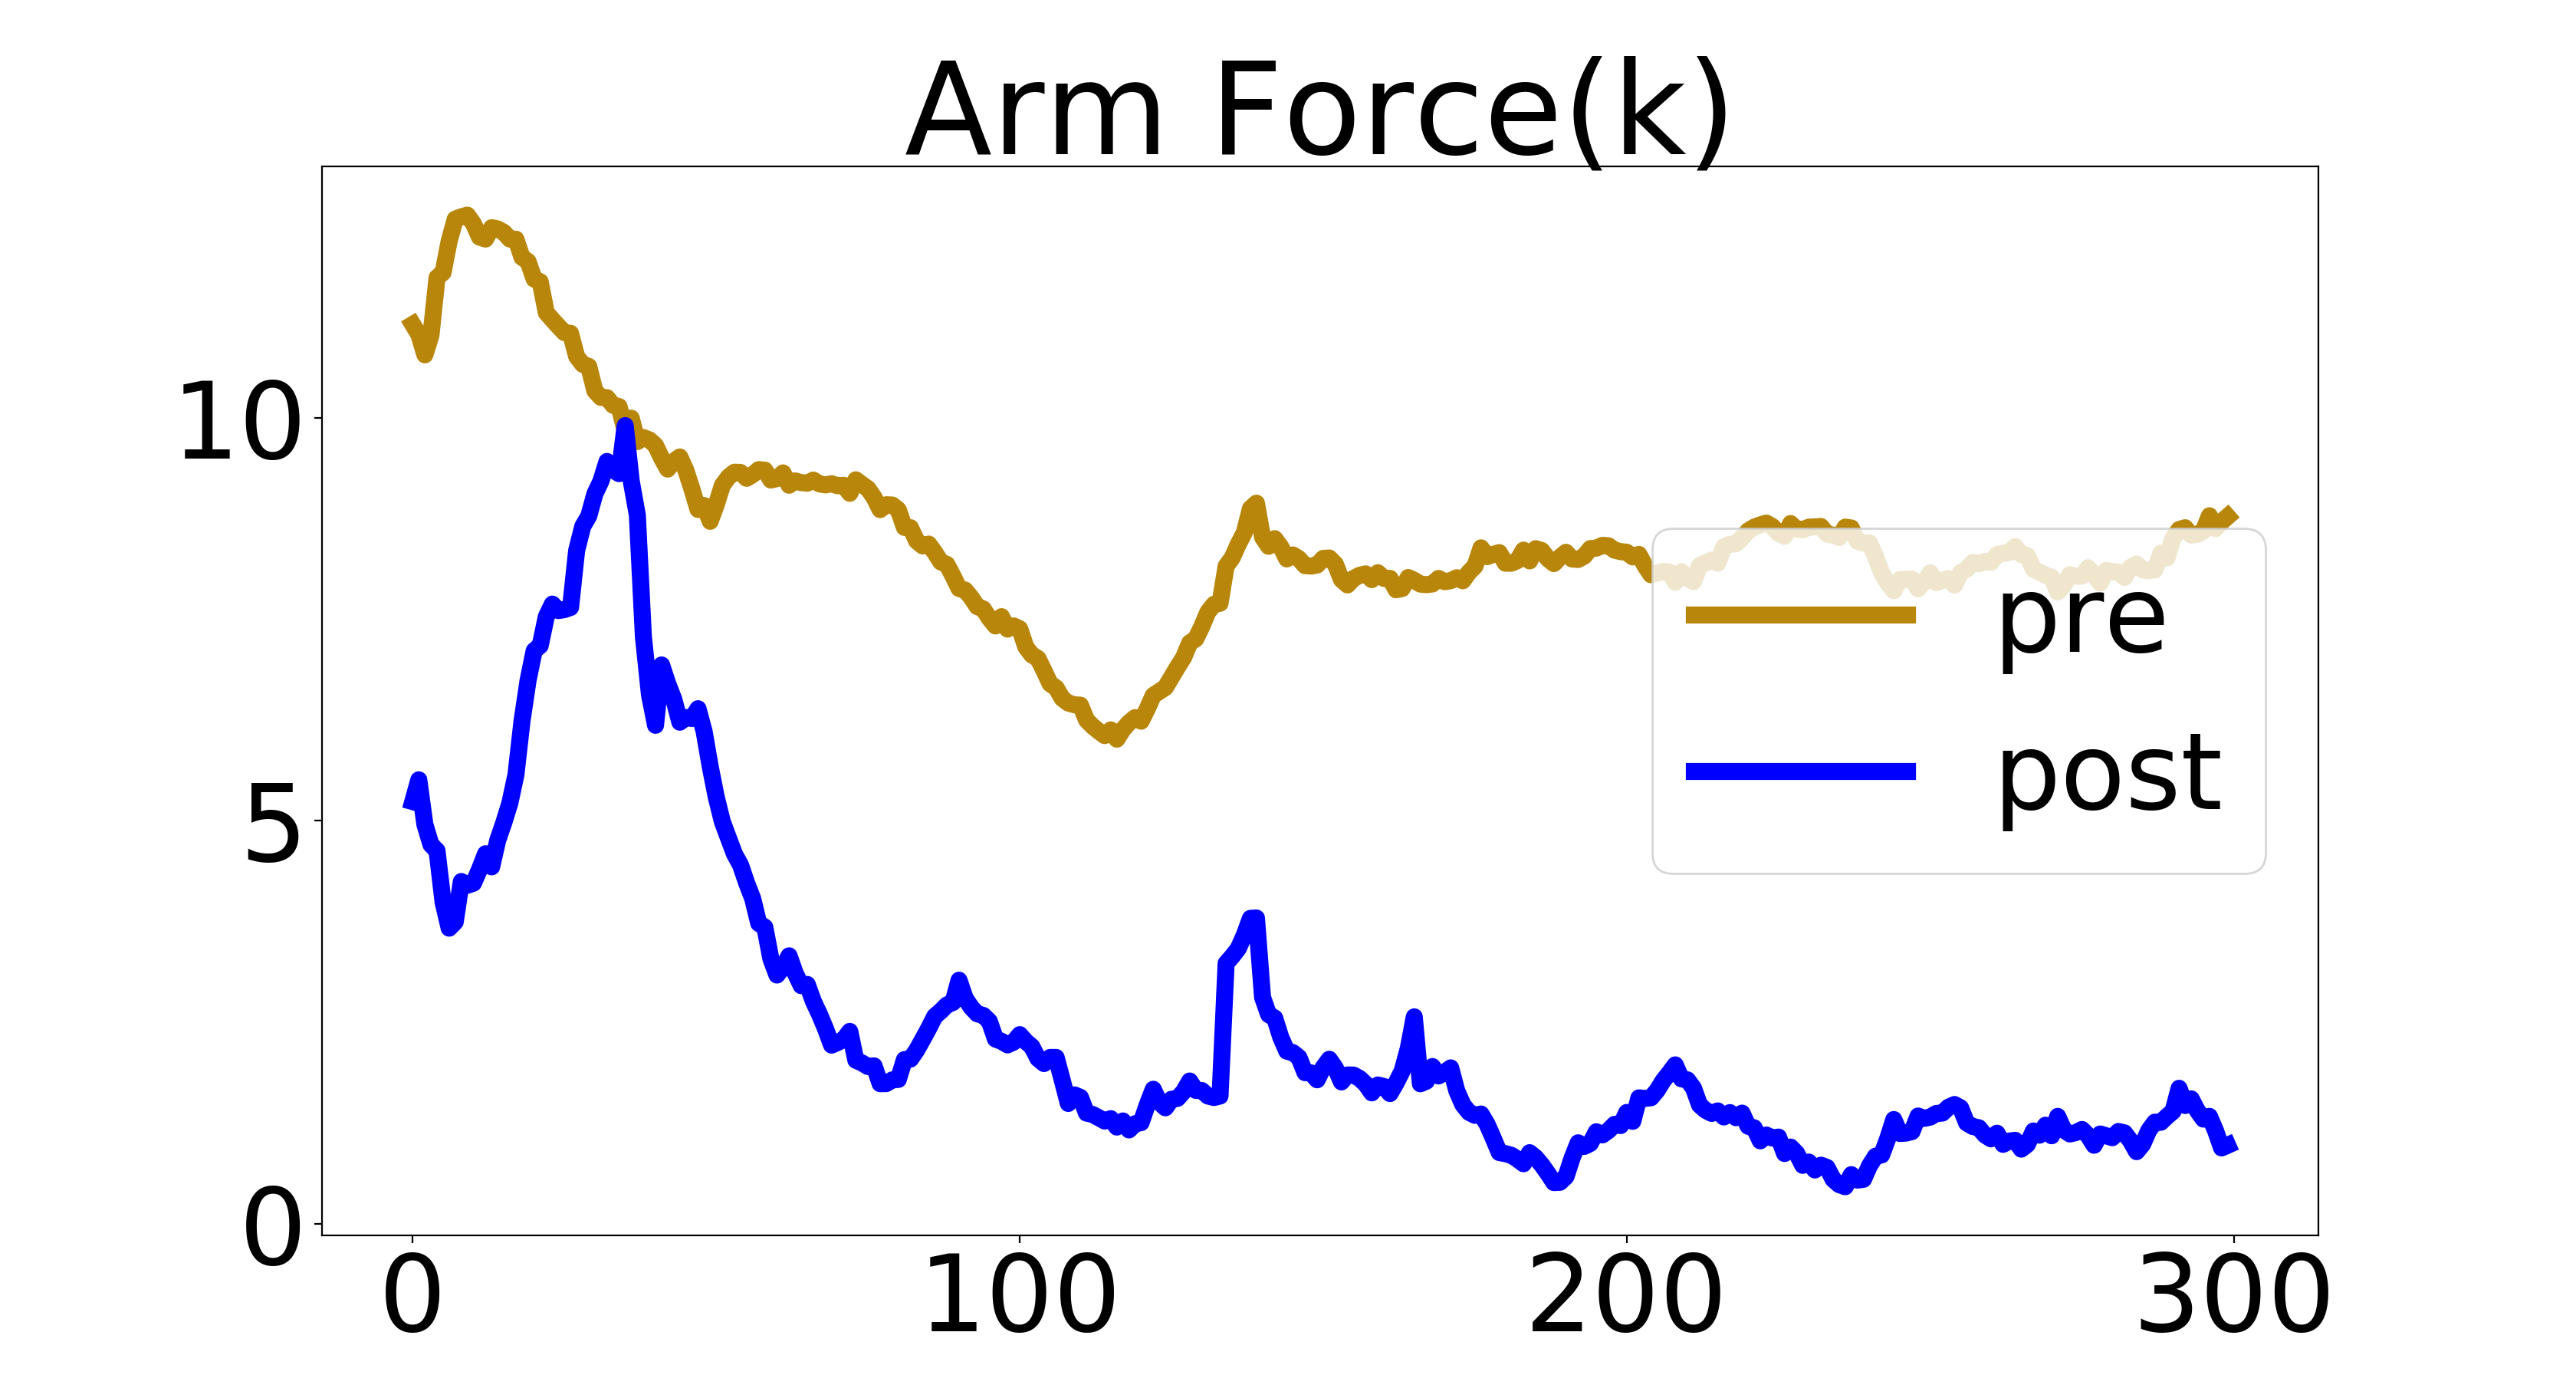
\includegraphics[width=0.3\textwidth]{pictures/errors_arm_task_k.png}
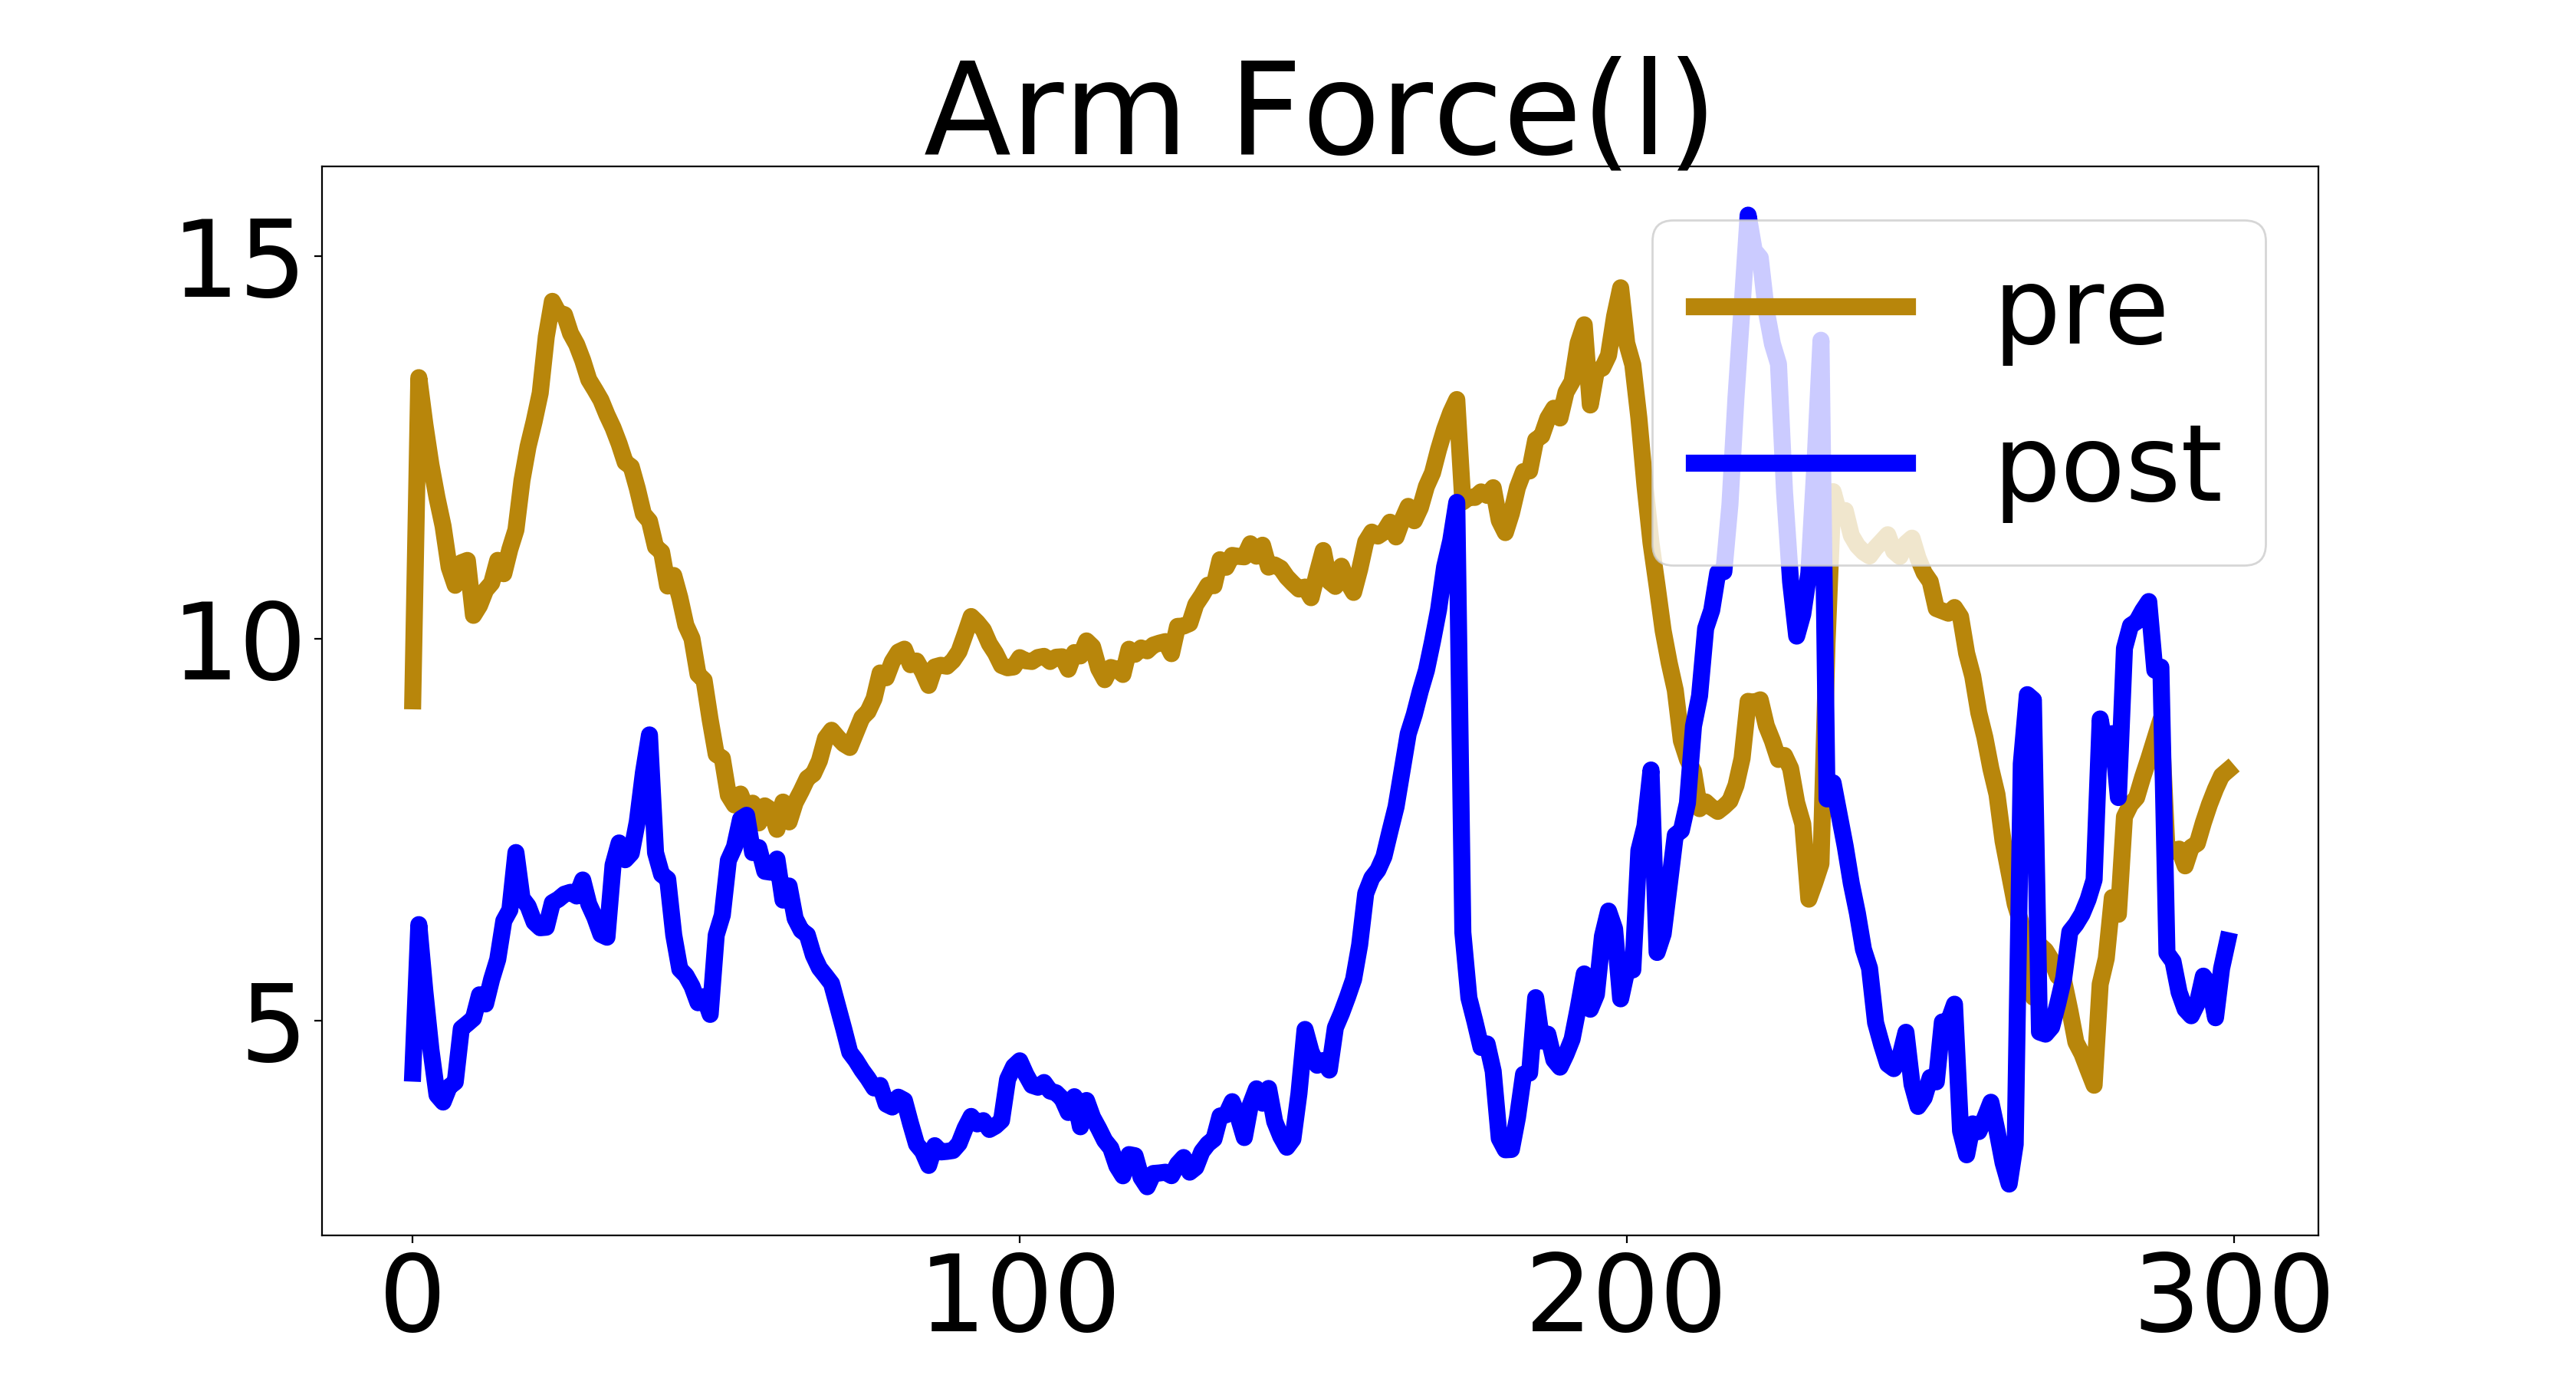
\includegraphics[width=0.3\textwidth]{pictures/error_arm_task_l.png}
\\
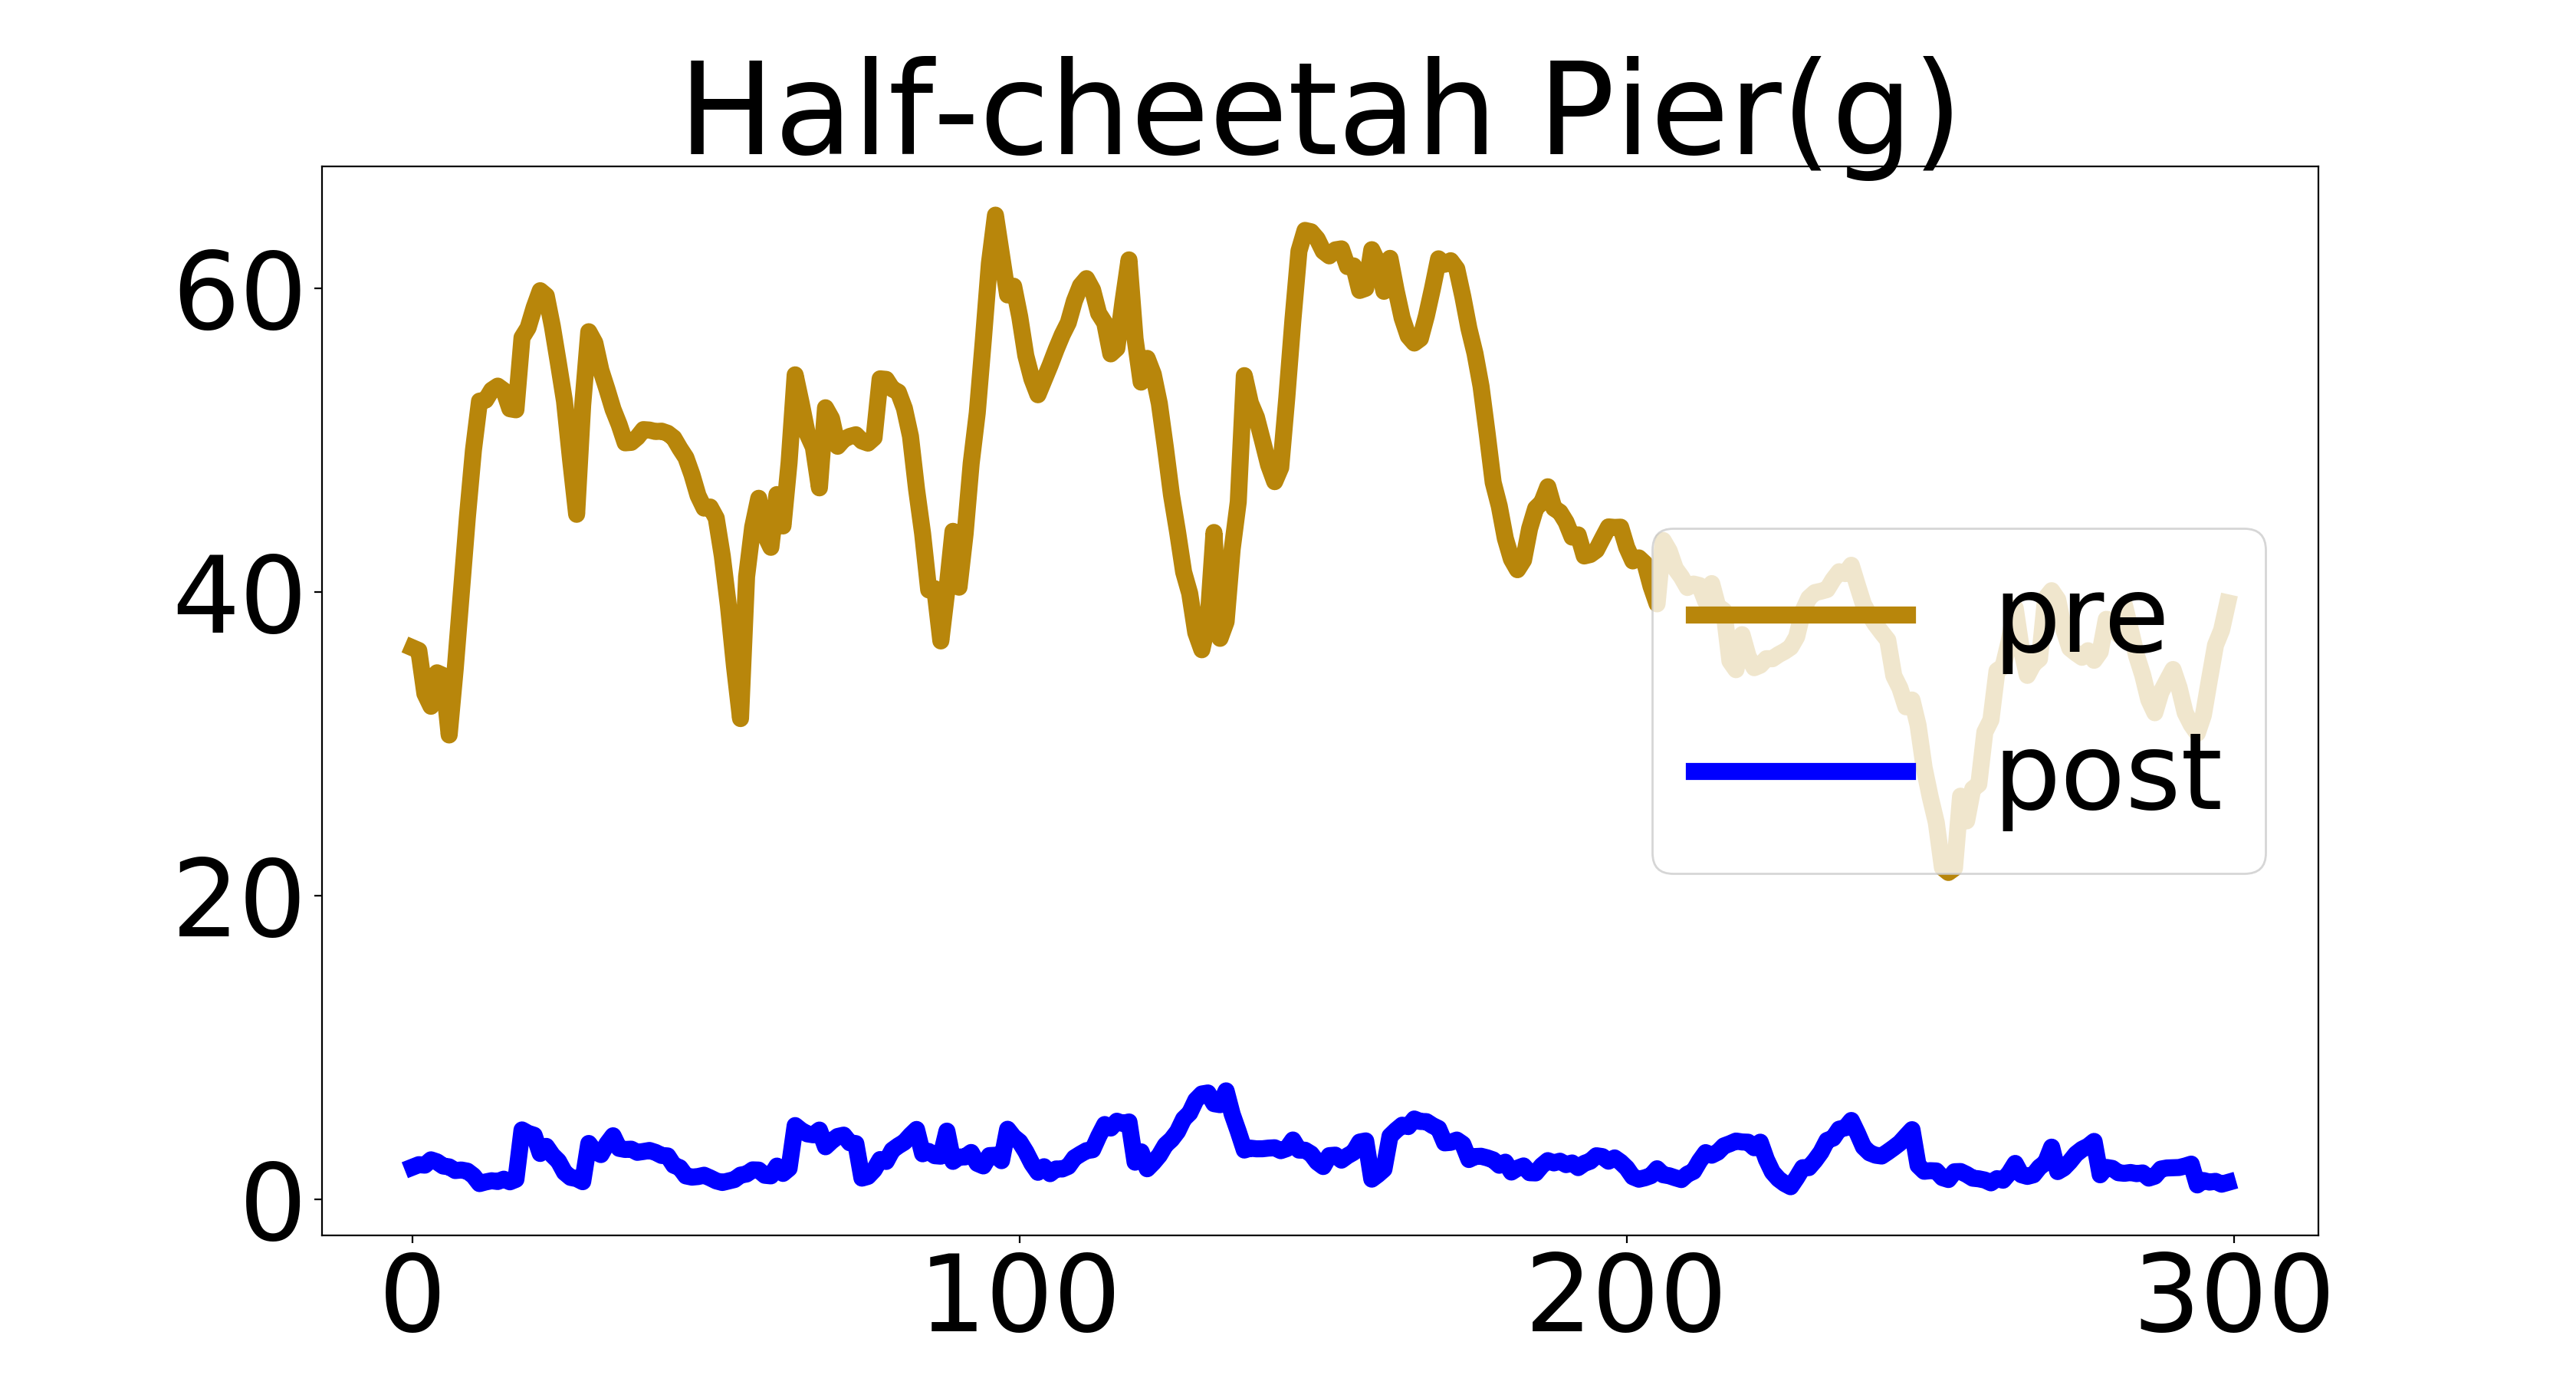
\includegraphics[width=0.3\textwidth]{pictures/error_hc_pier.png}
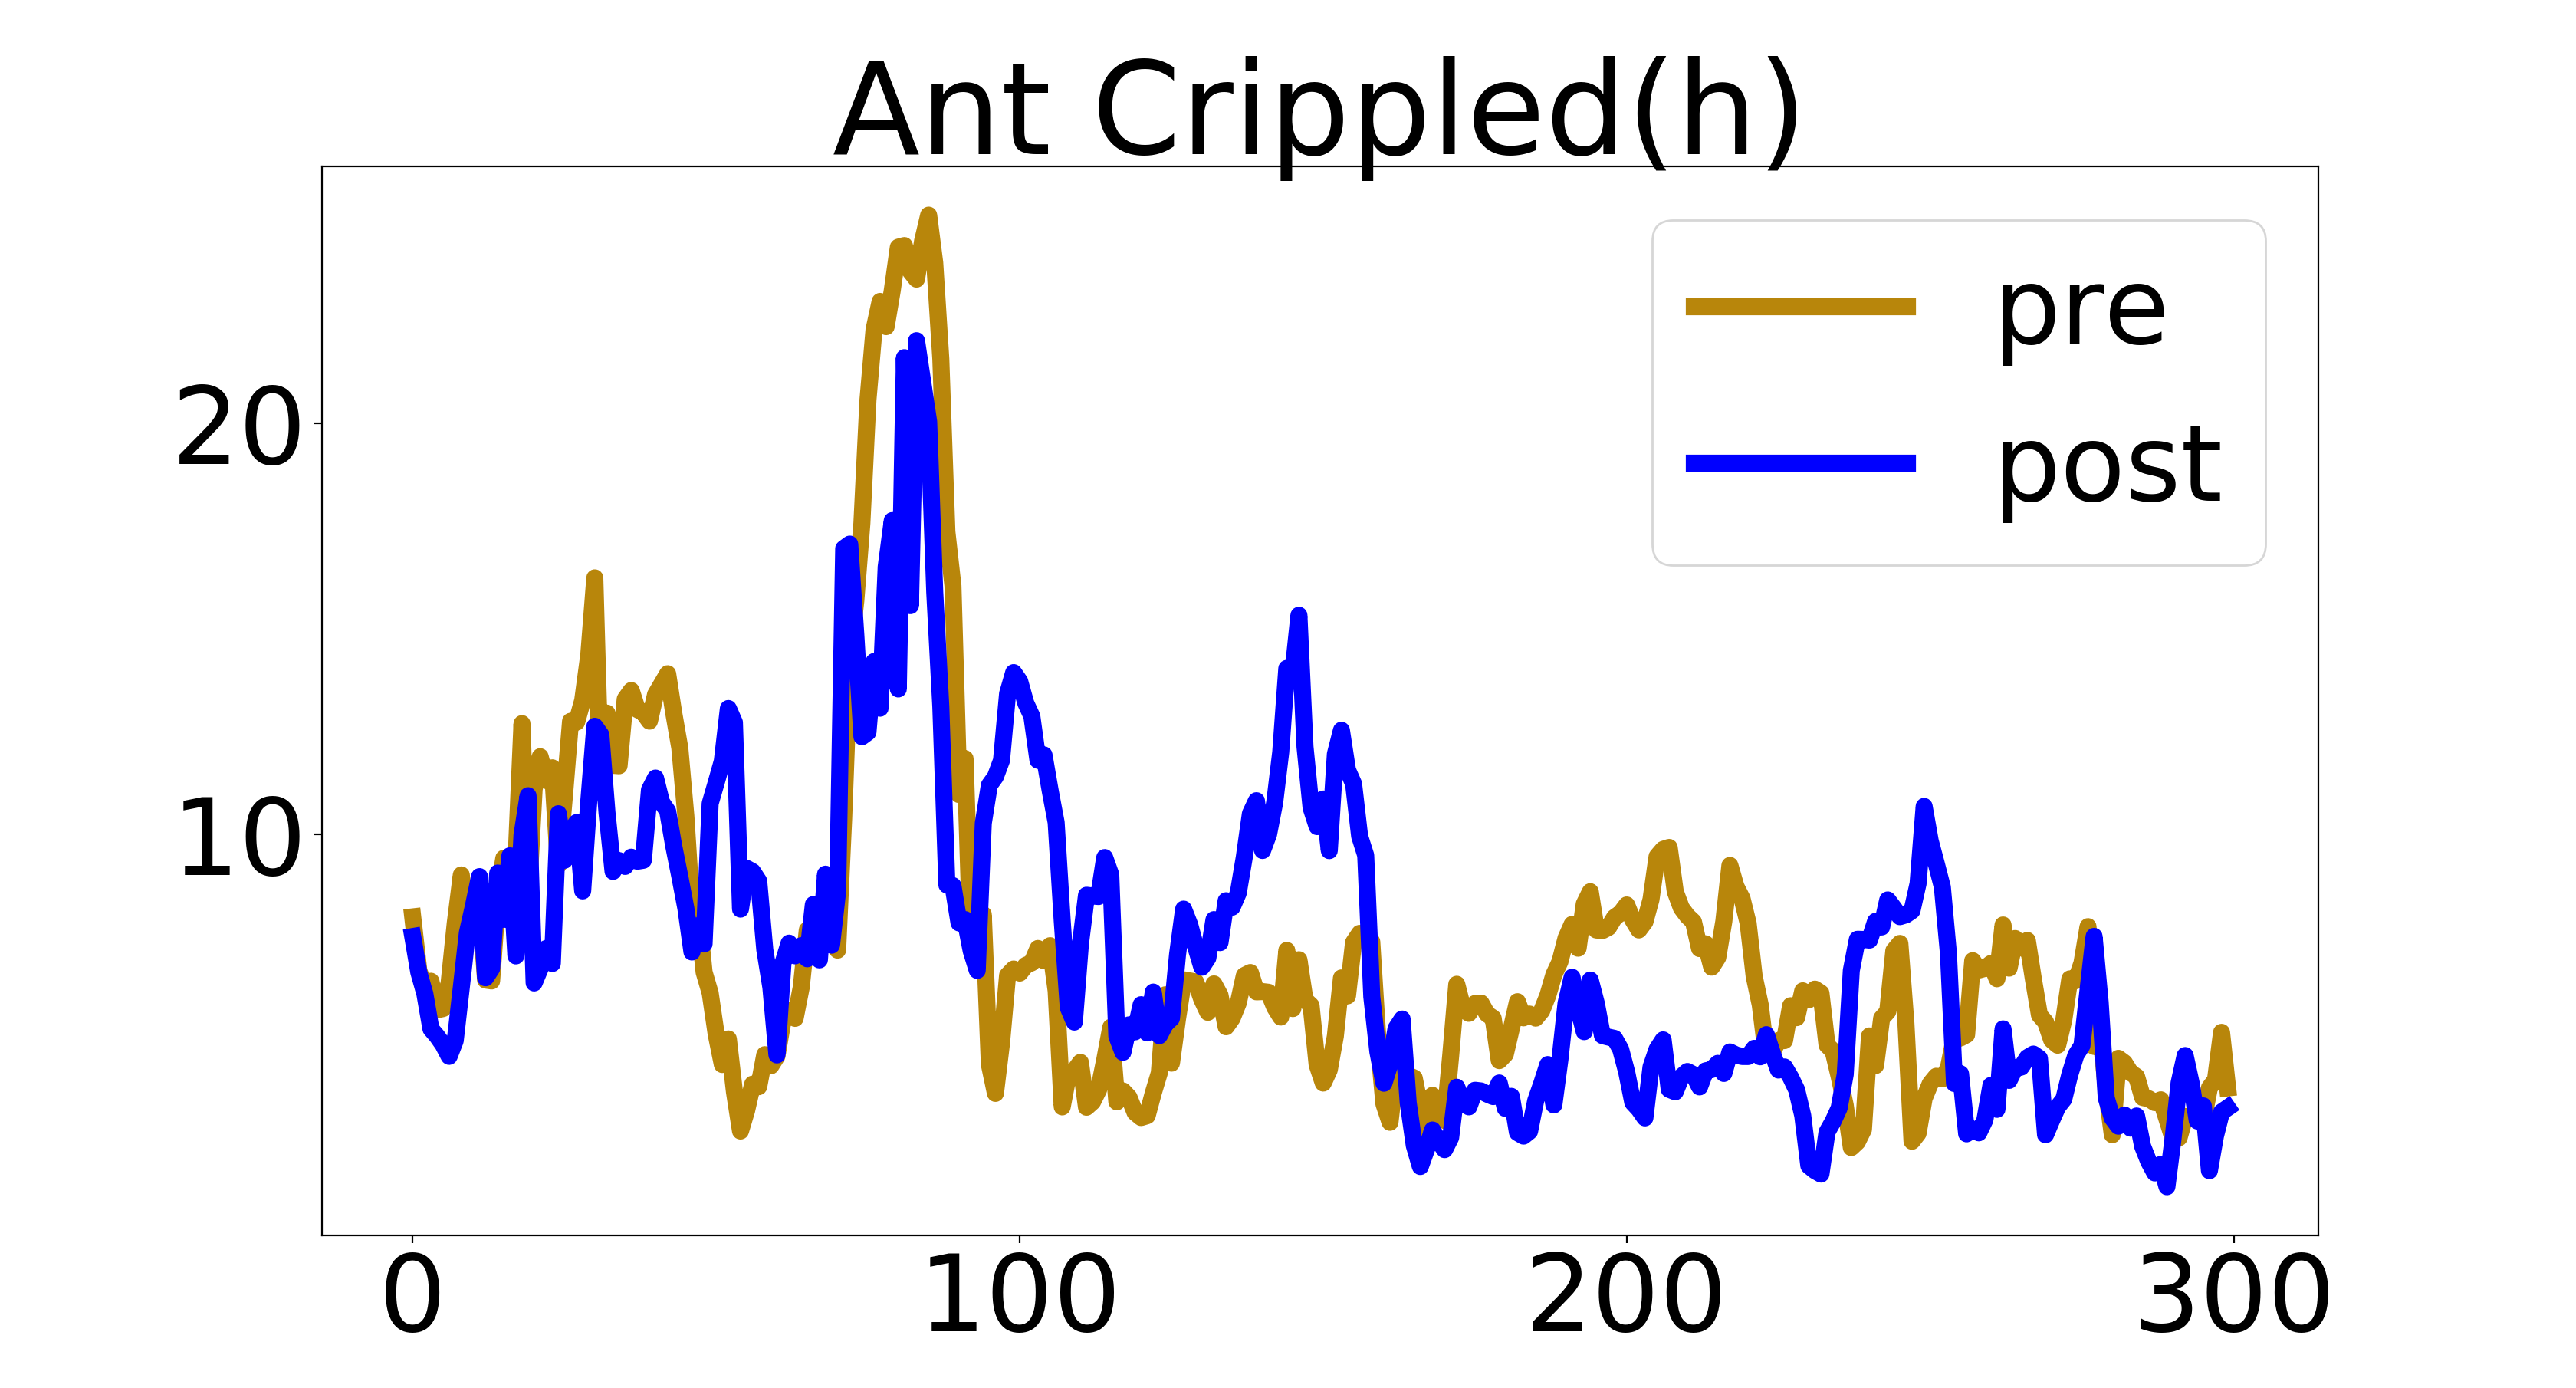
\includegraphics[width=0.3\textwidth]{pictures/error_ant_task_h.png}
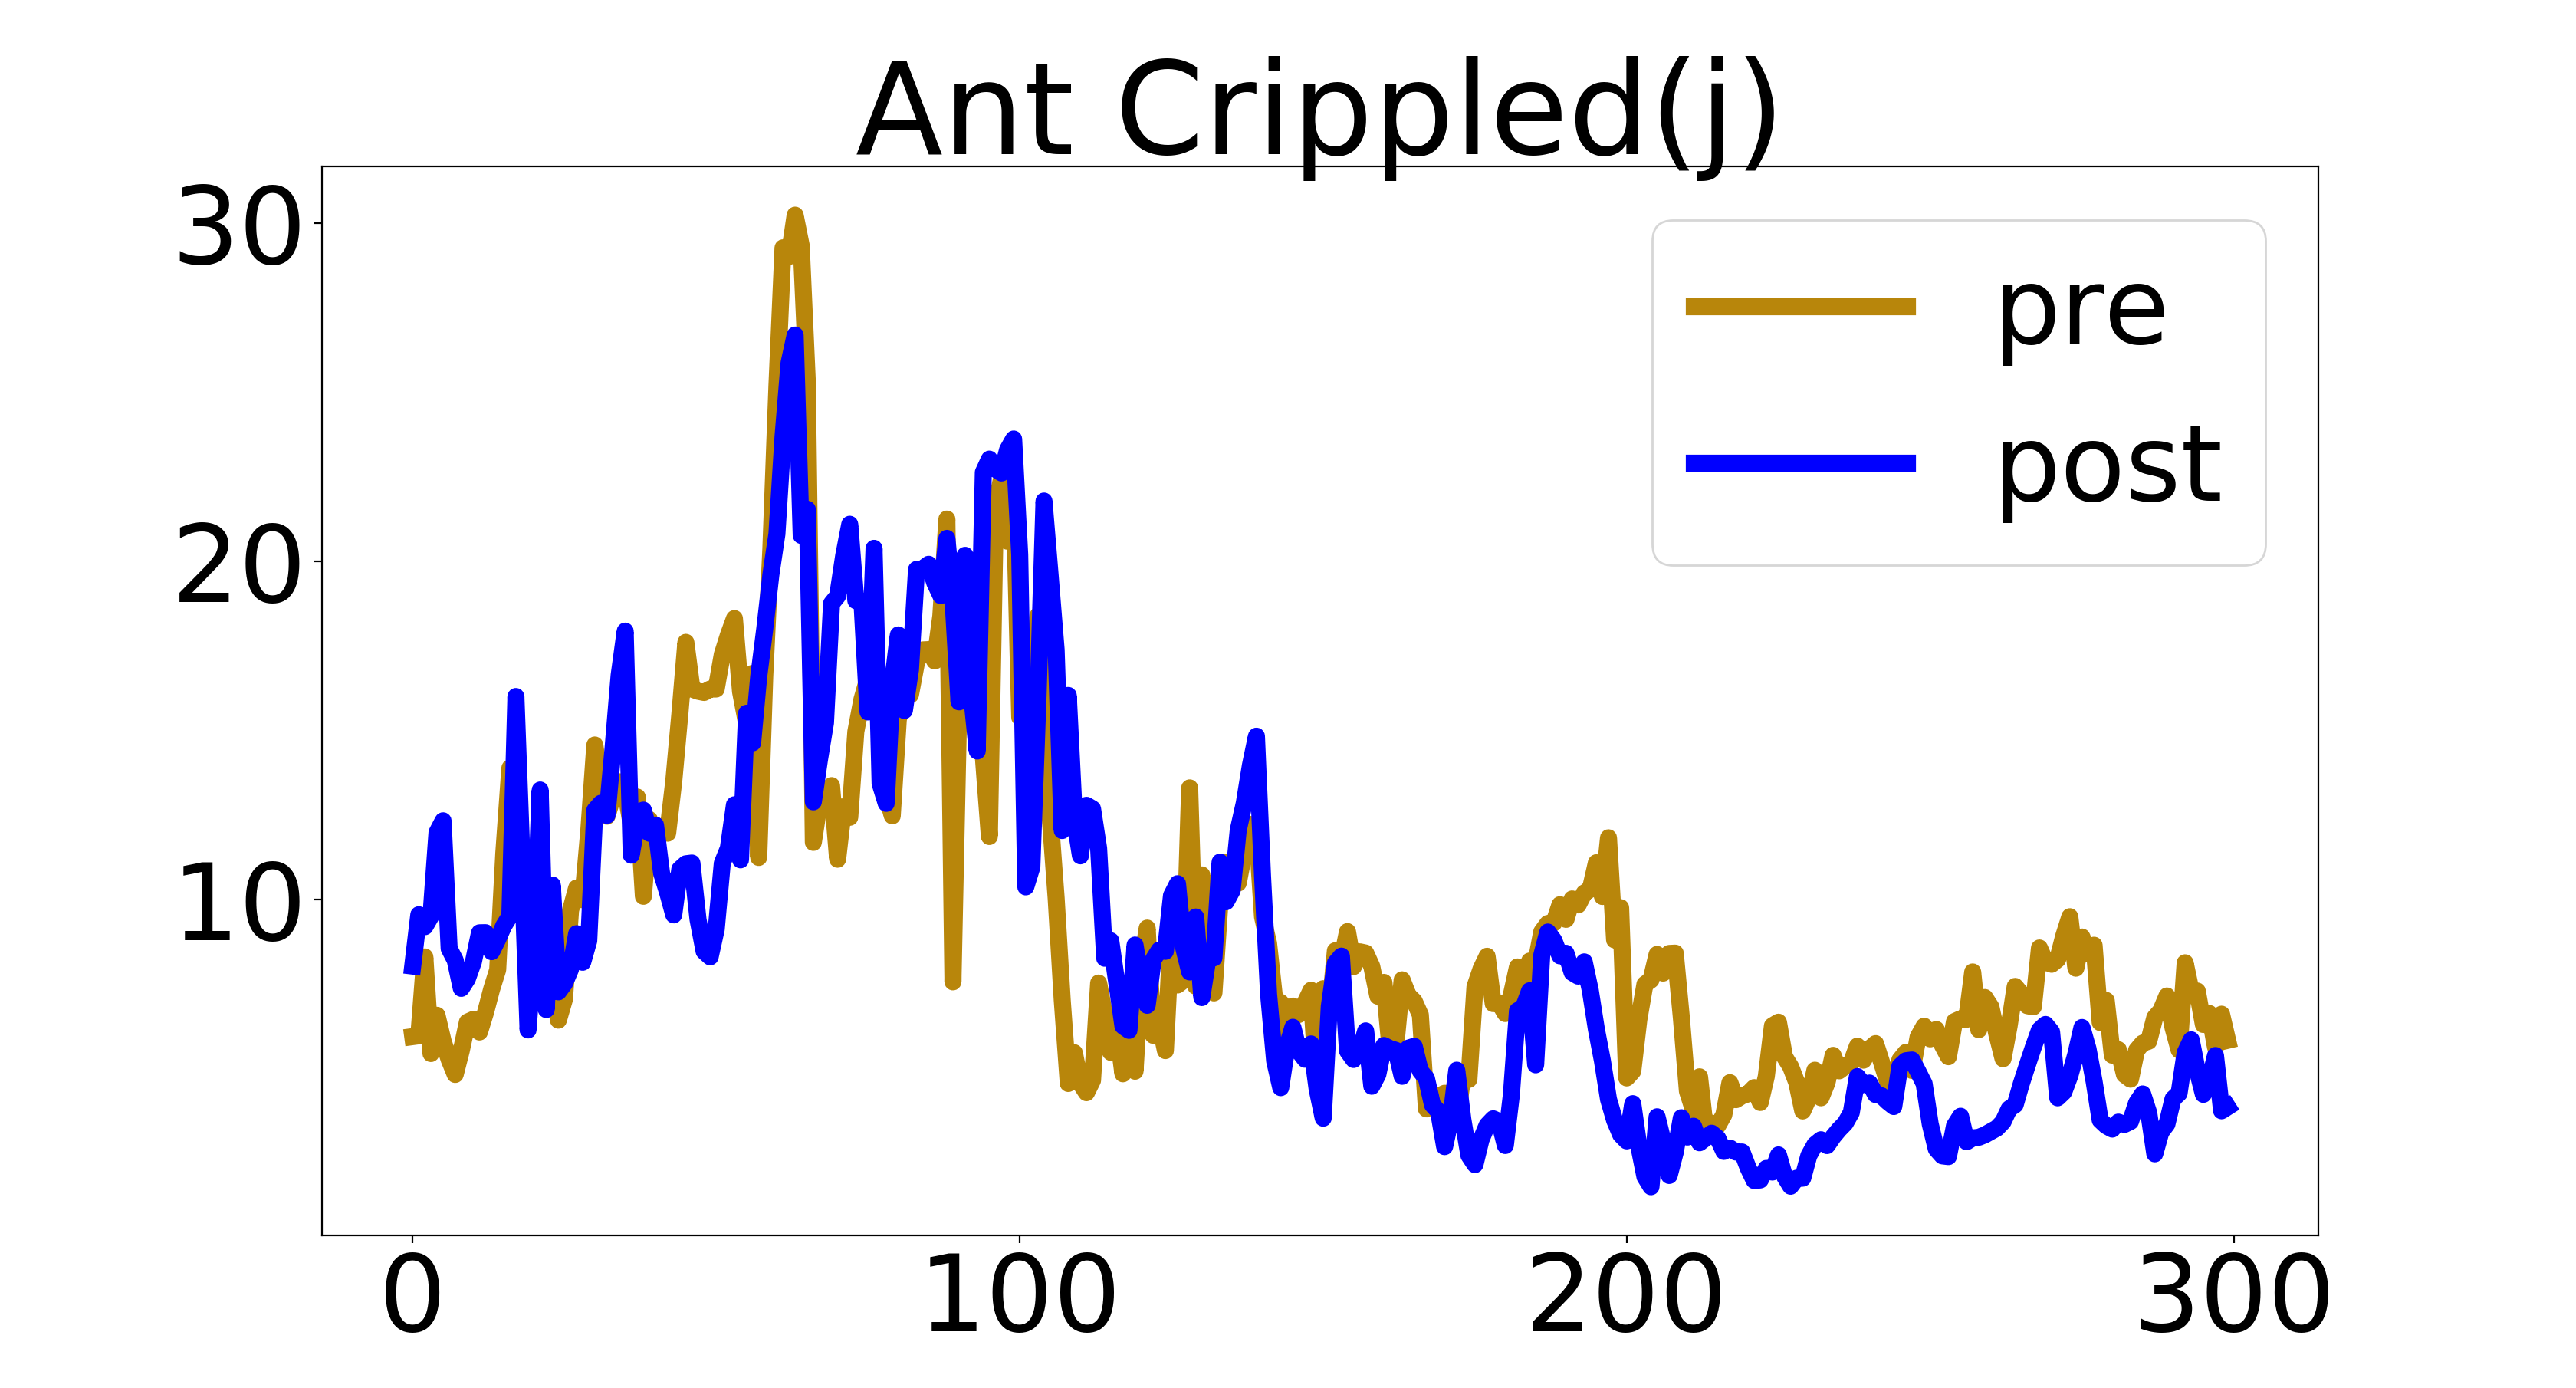
\includegraphics[width=0.3\textwidth]{pictures/error_ant_task_j.png}
\\
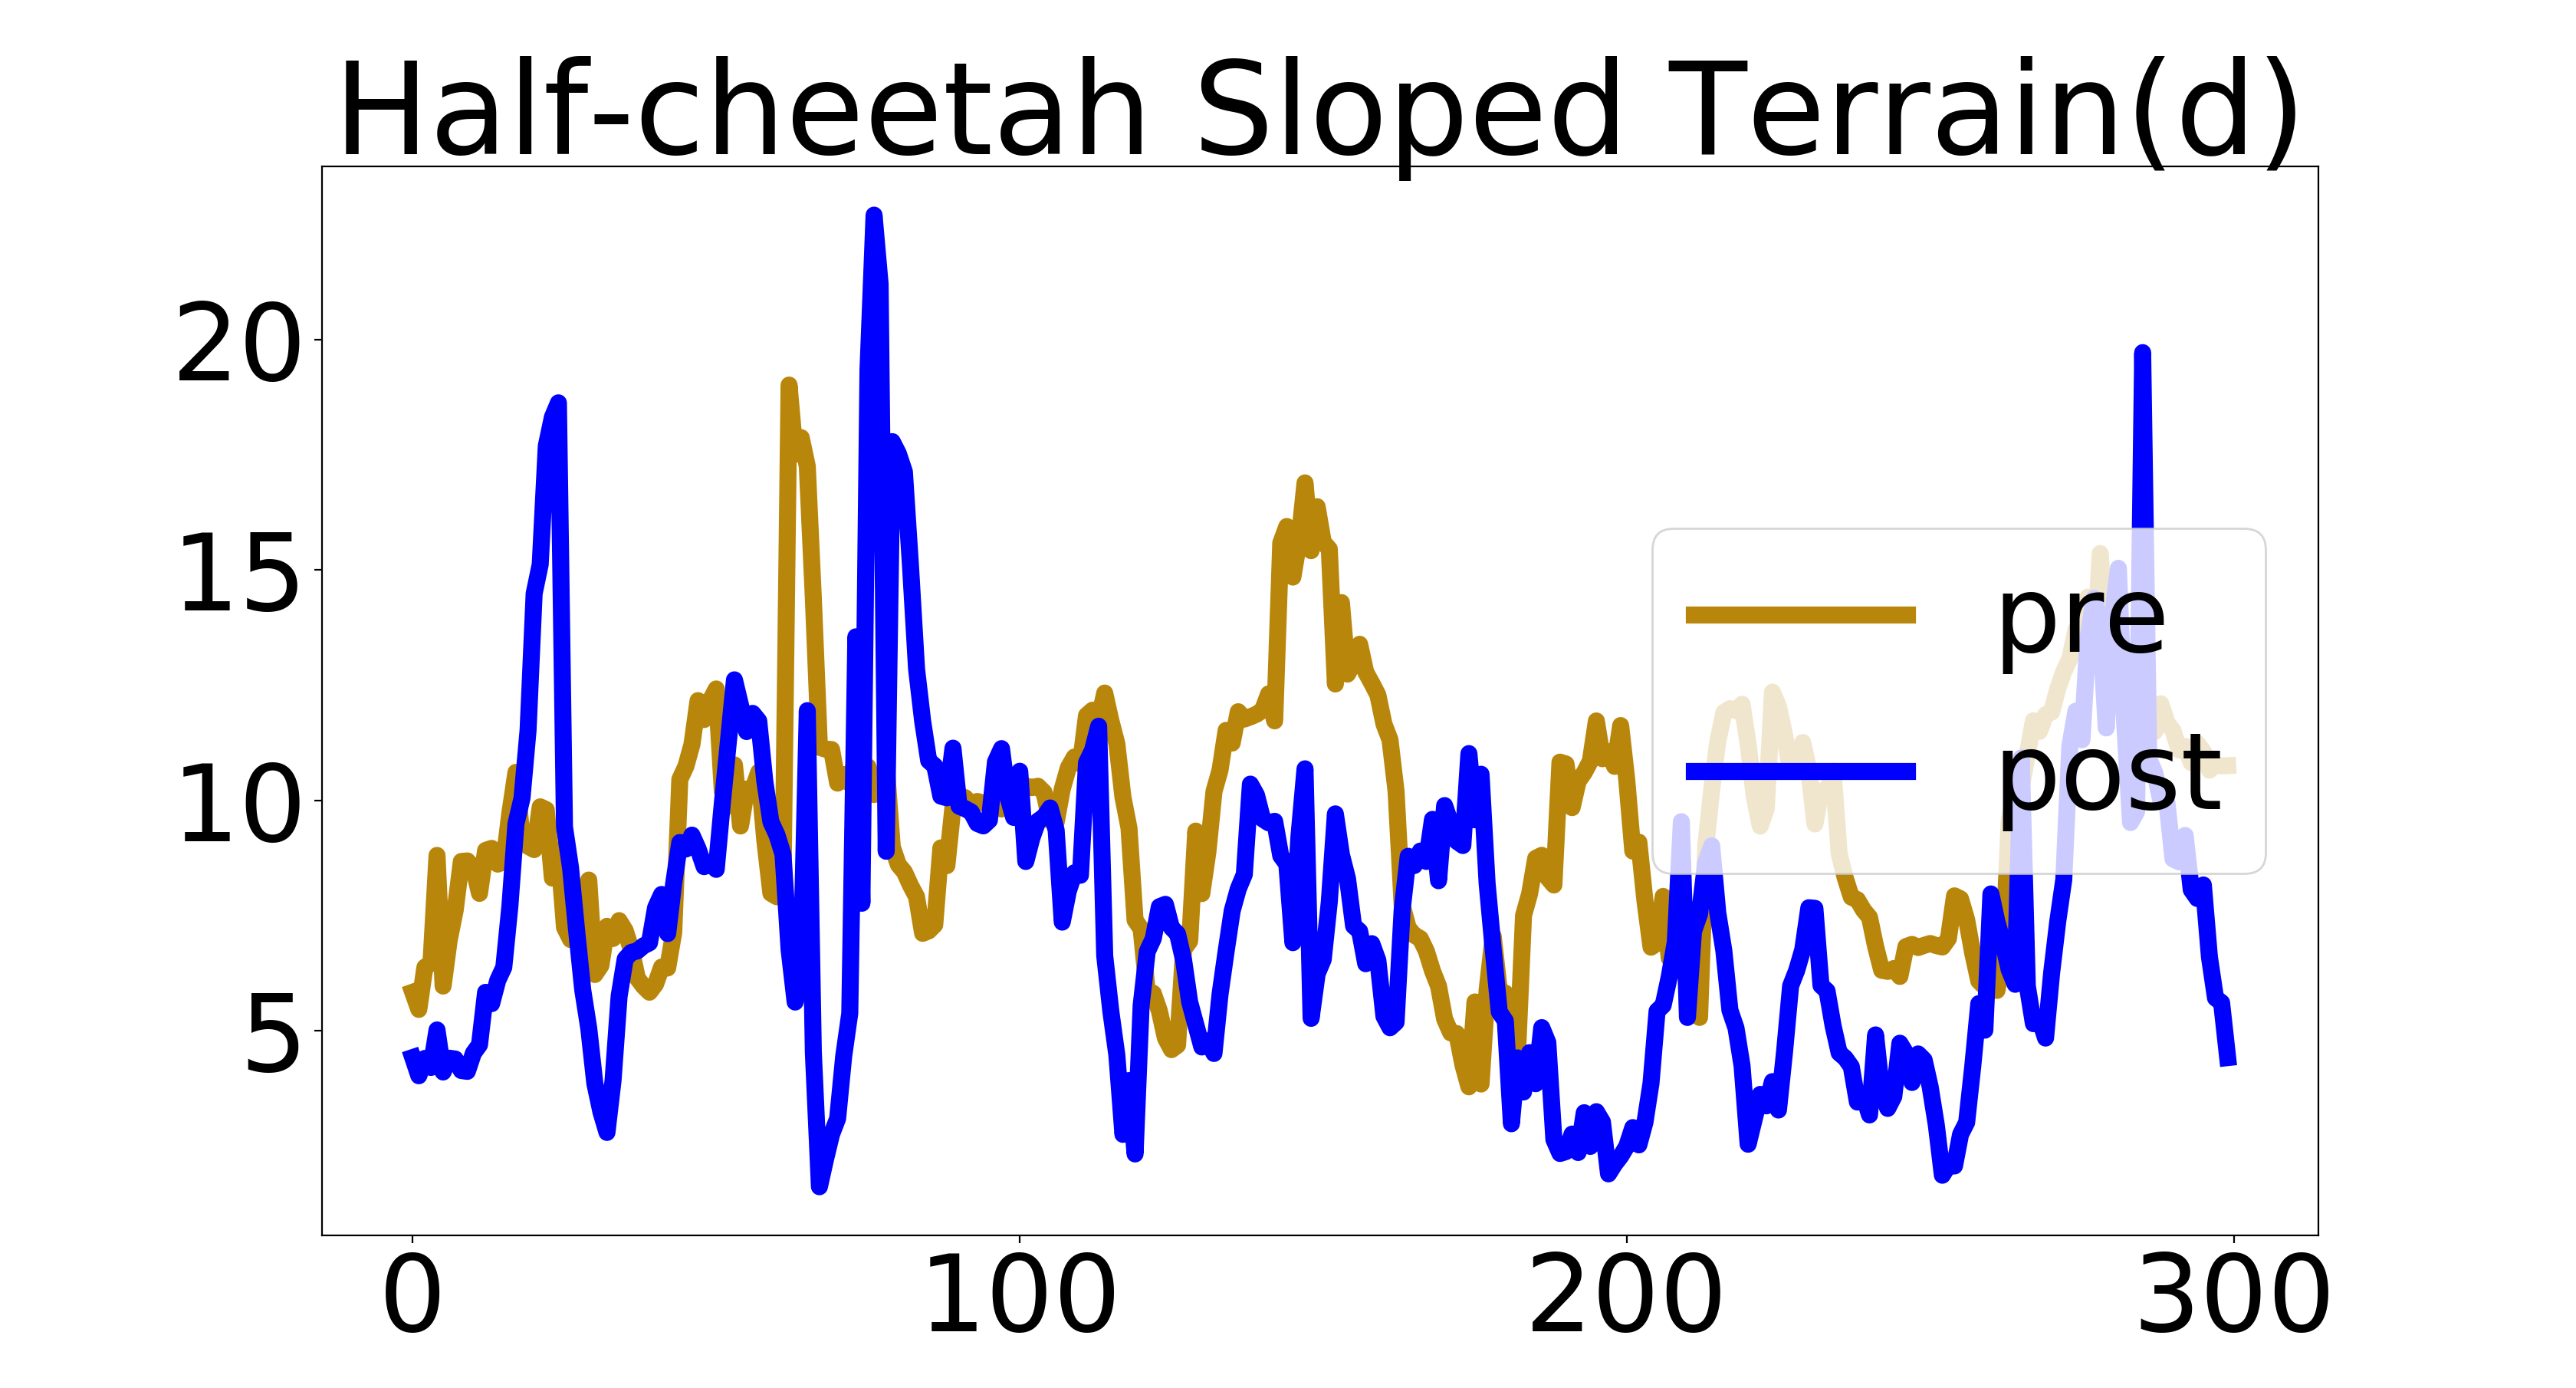
\includegraphics[width=0.3\textwidth]{pictures/error_hc_gentle.png}
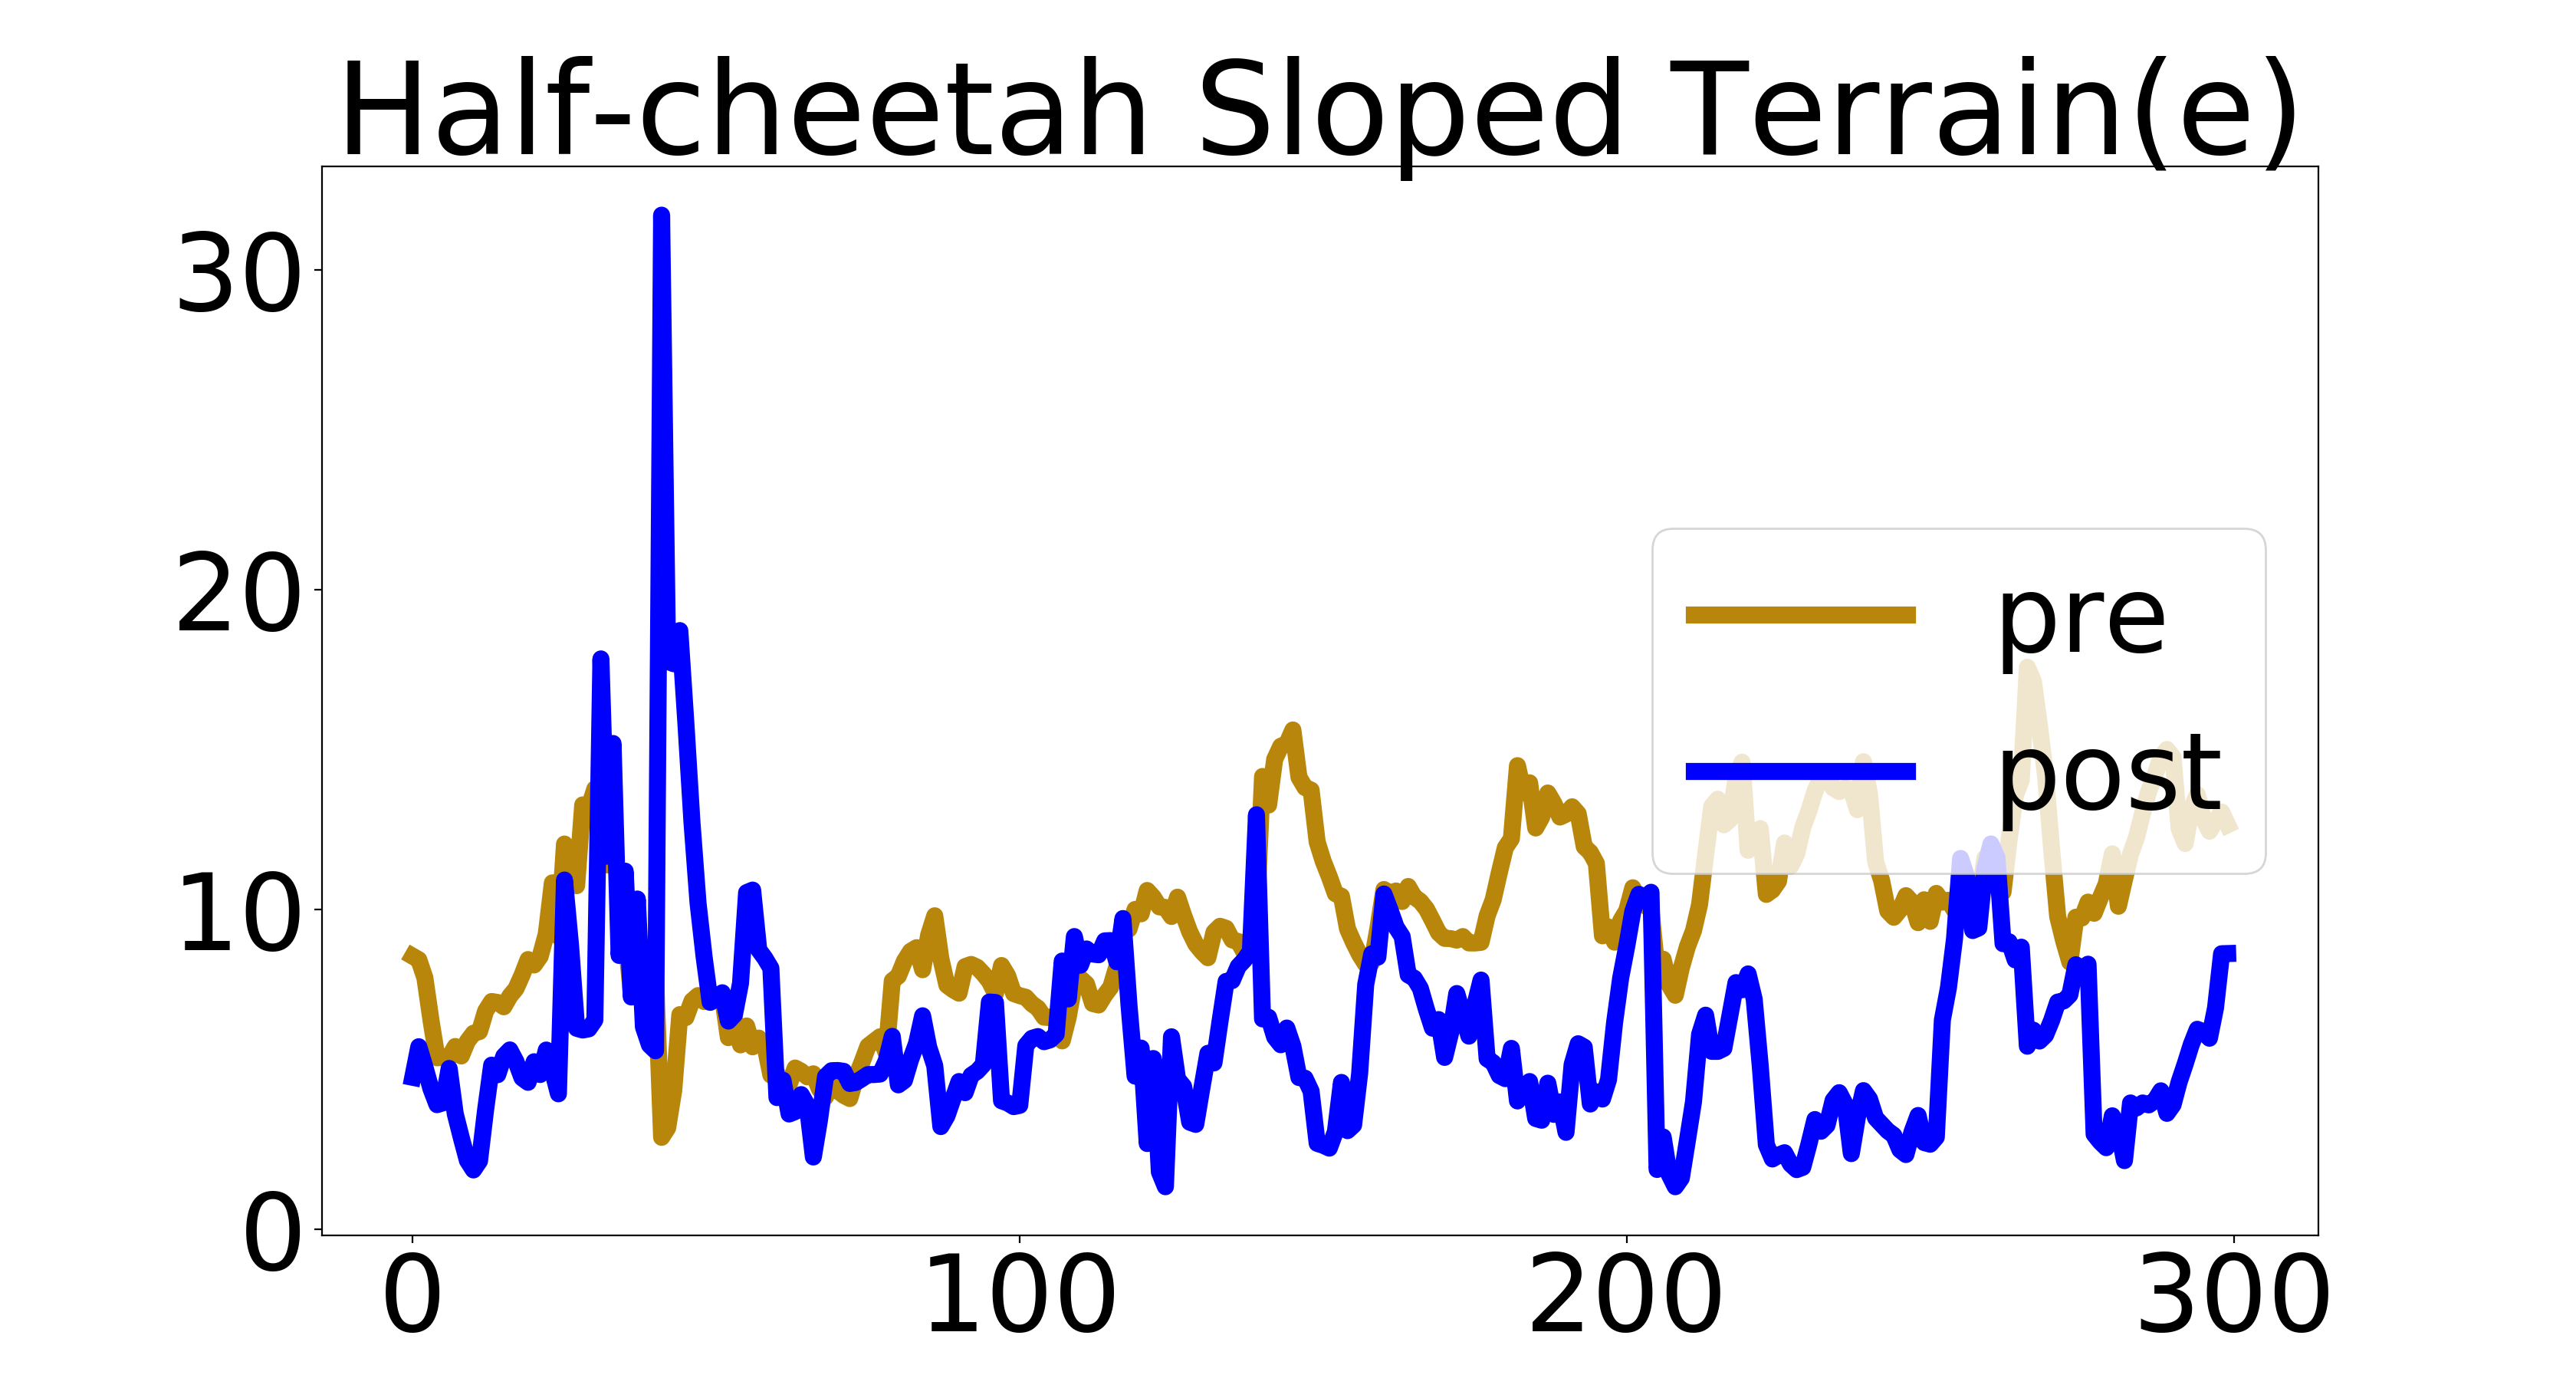
\includegraphics[width=0.3\textwidth]{pictures/error_hc_hill.png}
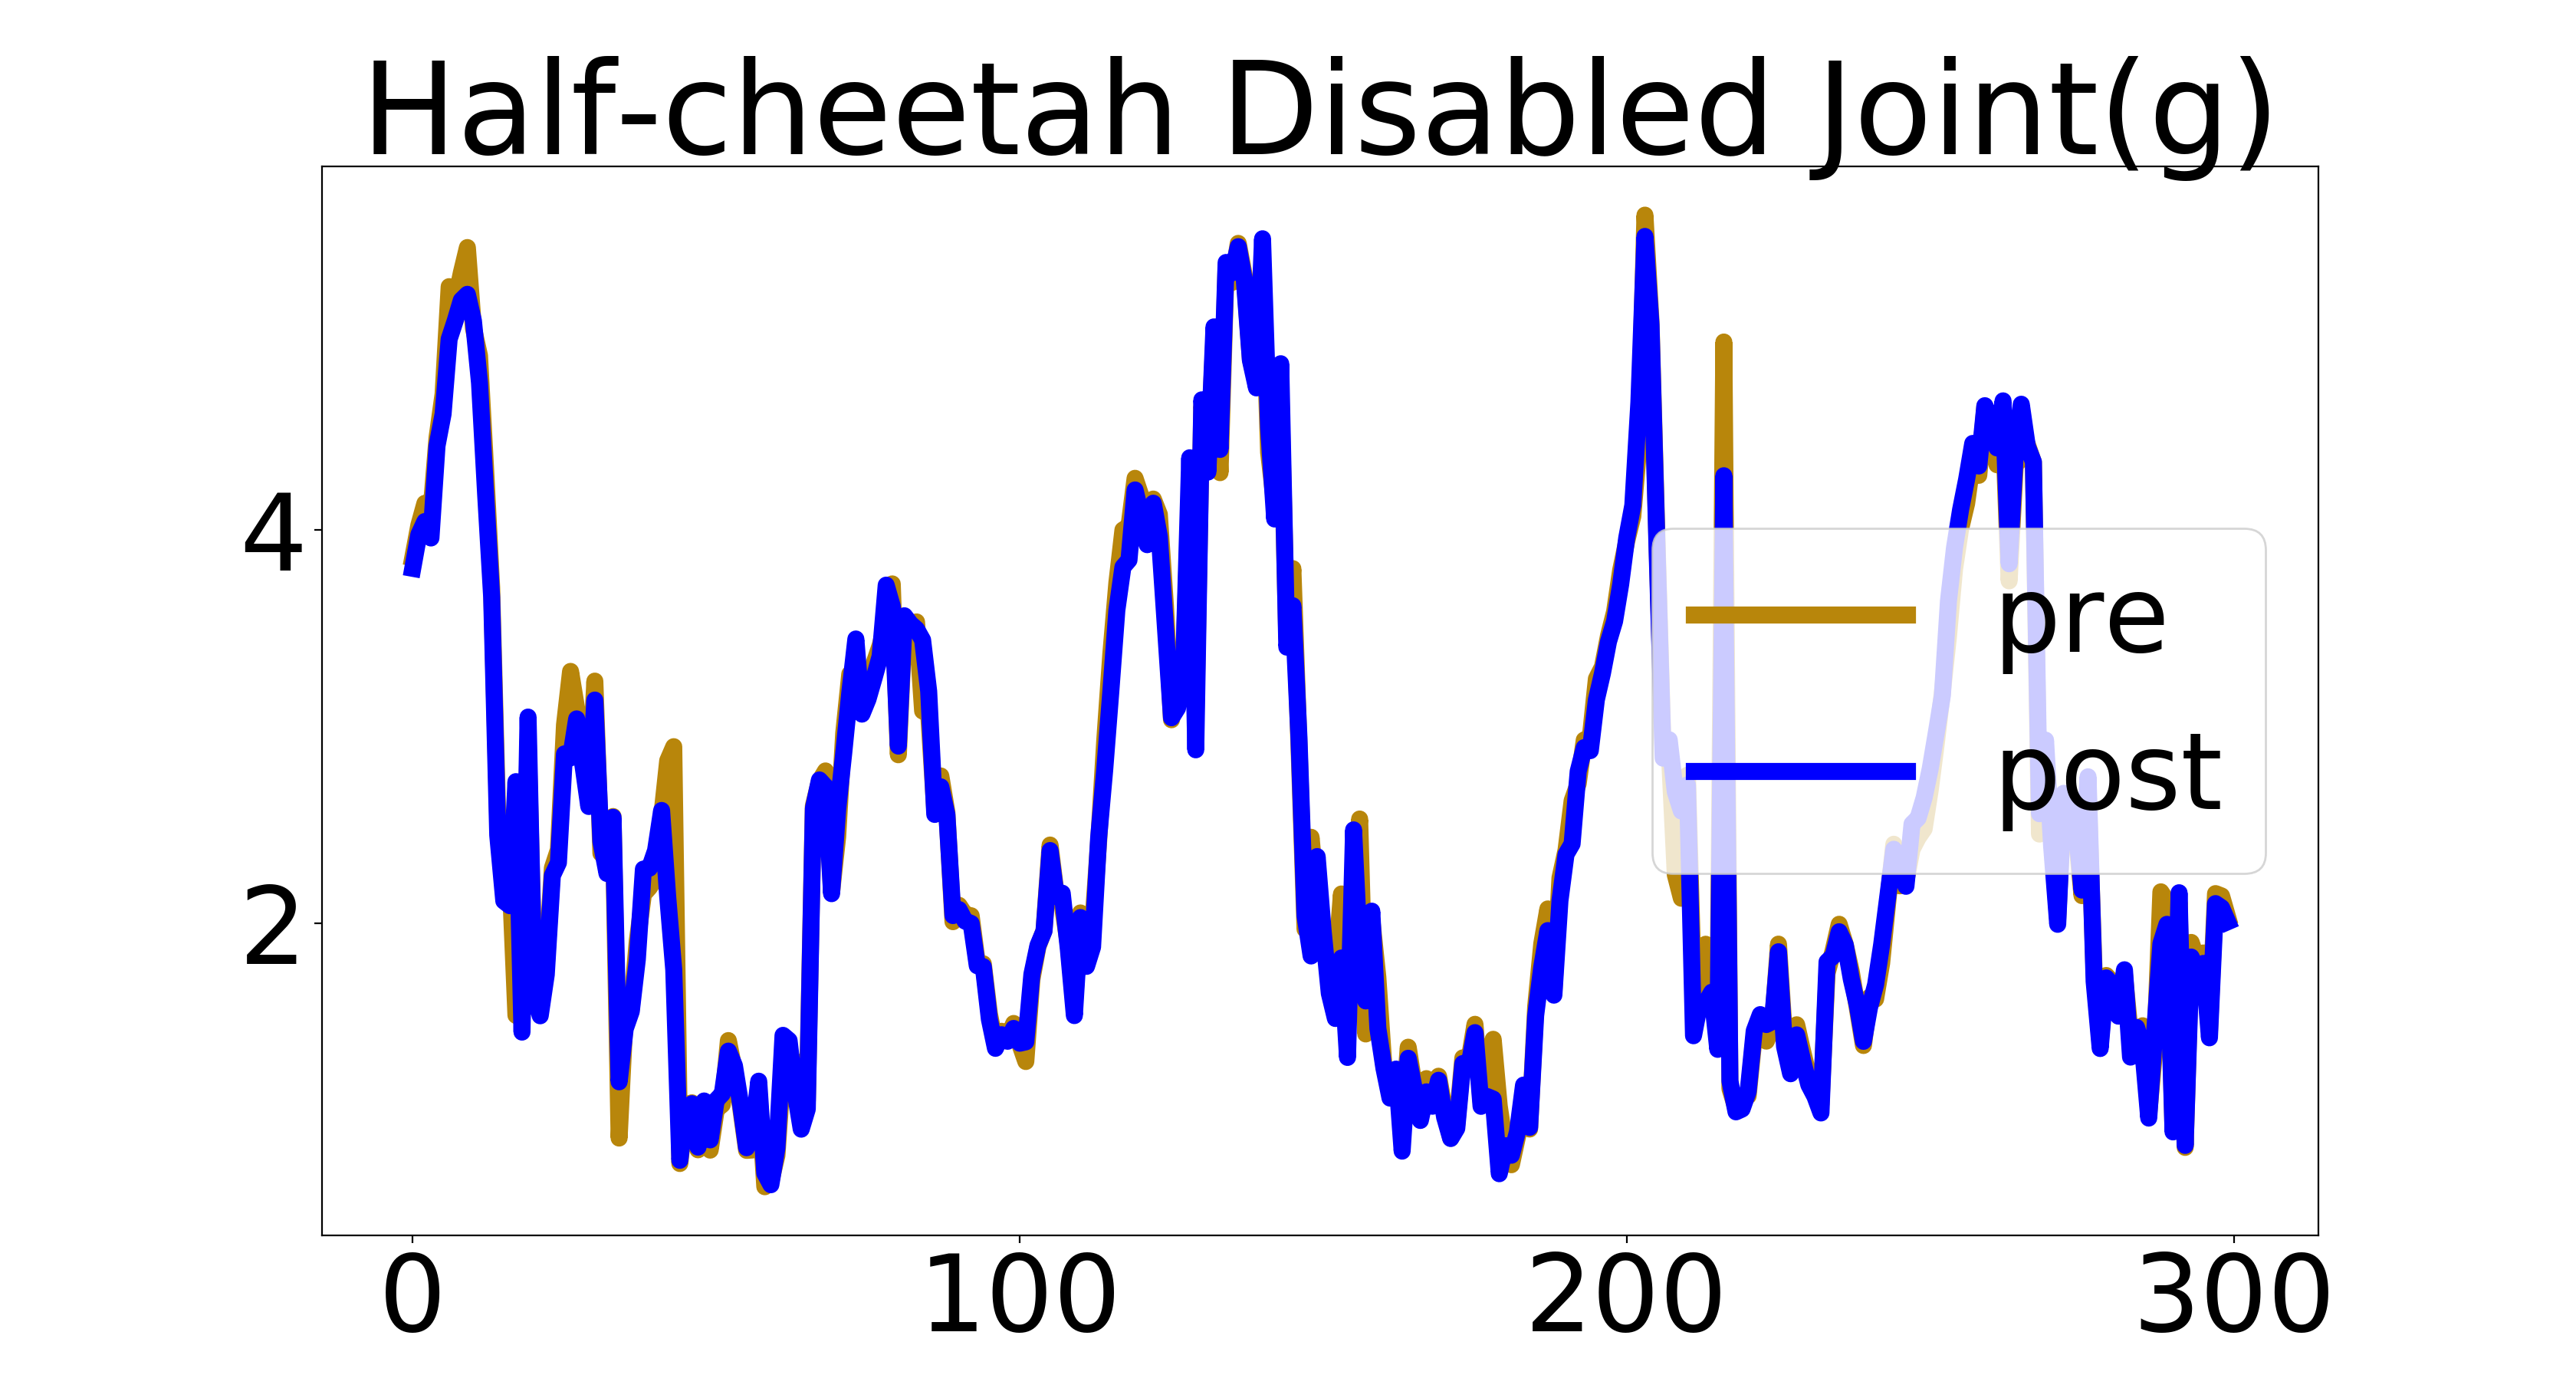
\includegraphics[width=0.3\textwidth]{pictures/error_hc_disabled.png}
% \vspace{-0.8cm}
% \vspace{-0.1in}
\caption{\small At each time-step we show the $K$ step normalized error across different tasks. GrBAL accomplishes lower model error using the parameters given by the update rule. }
\label{fig:errors} 
% \vspace{-0.2in}
\end{figure}


\newpage
\section{Effect of Meta-Training Distribution}

To see how training distribution affects test performance, we ran an experiment that used GrBAL to train models of the 7-DOF arm, where each model was trained on the same number of datapoints during meta-training, but those datapoints came from different ranges of force perturbations. We observe (in the plot below) that 

1. Seeing more during training is helpful during testing --- a model that saw a large range of force perturbations during training performed the best

2. A model that saw no perturbation forces during training did the worst

3. The middle 3 models show comparable performance in the "constant force = 4" case, which is an out-of-distribution task for those models. Thus, there is not actually a strong restriction on what needs to be seen during training in order for adaptation to occur at train time (though there is a general trend that more is better)

\begin{figure}
\centering
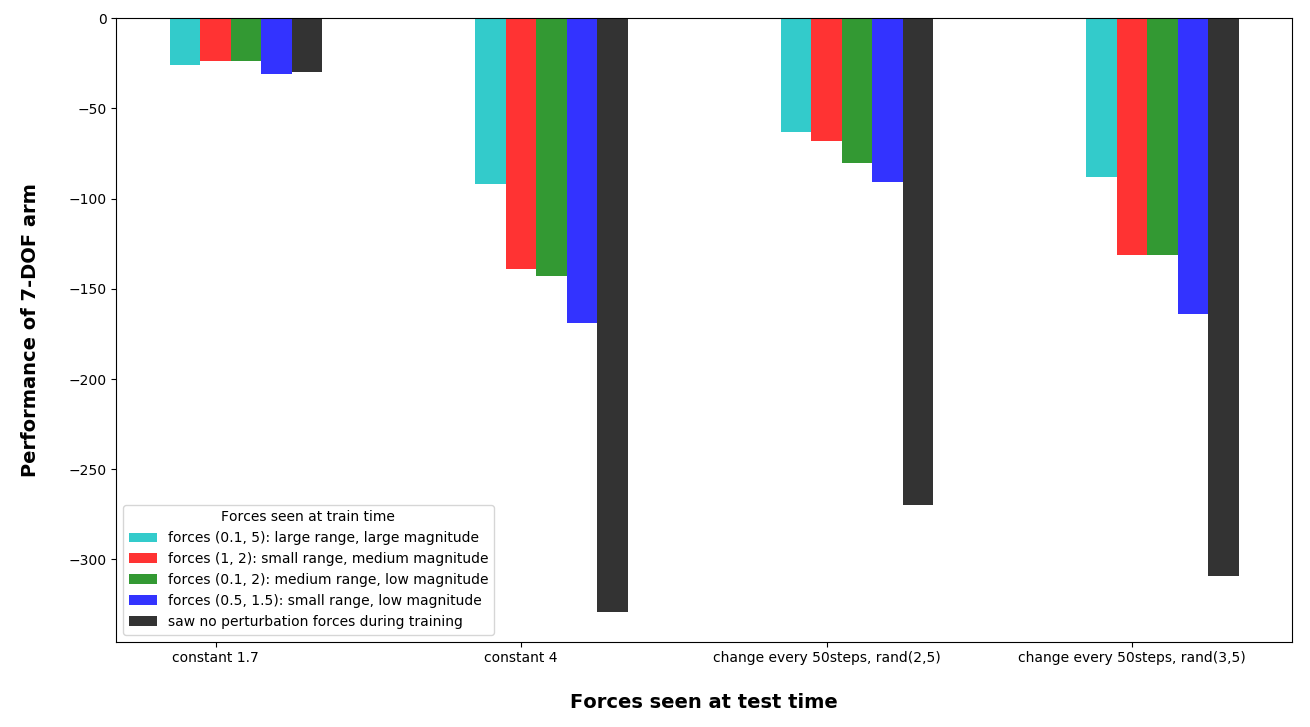
\includegraphics[width=\columnwidth]{pictures/metatrainingdistrib.png}
\caption{Effect of the meta-training distribution on test performance}
\label{fig:metatrainingdistrib}
\end{figure}

\newpage
\section{Sensitivity of K and M}
In this section we analyze how sensitive is our algorithm w.r.t the hyperparameters $K$ and $M$. In all experiments of the paper, we set $K$ equal to $M$.  Figure~\ref{fig:sensitivity} shows the average return of GrBAL across meta-training iterations of our algorithm for different values of $K=M$. The performance of the agent is largely unaffected for different values of these hyperparameters, suggesting that our algorithm is not particularly sensitive to these values. For different agents, the optimal value for these hyperparameters depends on various task details, such as the amount of information present in the state (a fully-informed state variable precludes the need for additional past timesteps) and the duration of a single timestep (a longer timestep duration makes it harder to predict more steps into the future). 


\begin{figure}[H]
\centering
% \vspace{-0.1in}
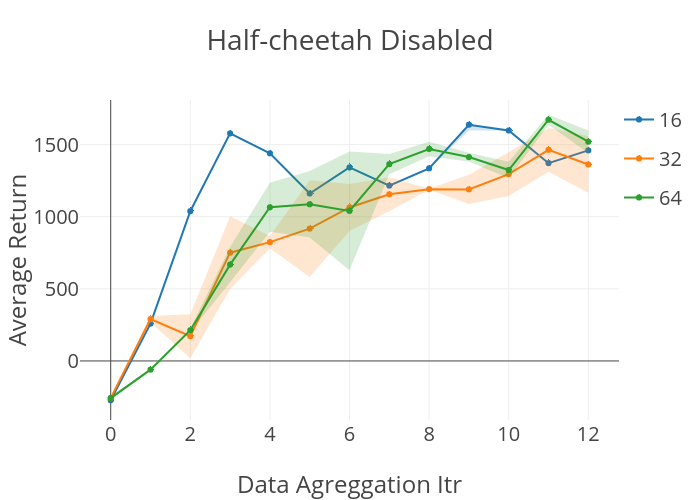
\includegraphics[width=0.45\textwidth]{pictures/half_cheetah_disabled.png}
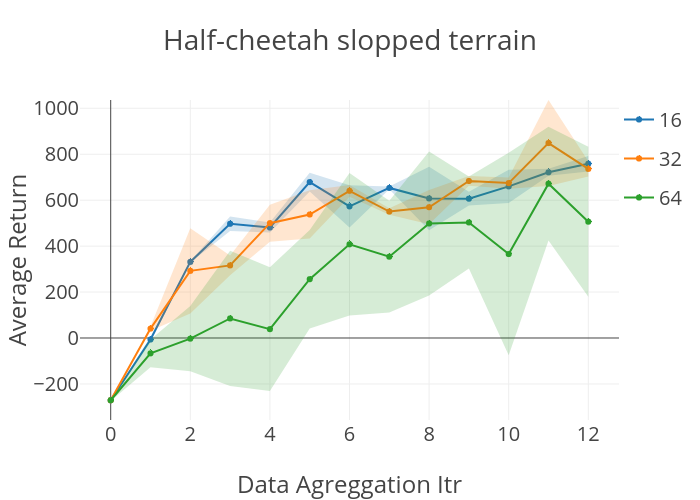
\includegraphics[width=0.45\textwidth]{pictures/half_cheetah_hfield.png}

\caption{\small Learning curves, for different values of $K=M$, of GrBAL in the half-cheetah disabled and sloped terrain environments. The x-axis shows data aggreation iterations during meta-training, whereas the y-axis shows the average return achieved when running online adaptation with the meta-learned model from the particular iteration. The curves suggest that GrBAL performance is fairly robust to the values of these hyperparameters. }
\label{fig:sensitivity}
% \vspace{-0.1in}
\end{figure}



\section{Reward functions}
For each MuJoCo agent, the same reward function is used across its various tasks. Table~\ref{tab:reward functions} shows the reward functions used for each agent. We denote by $x_t$ the x-coordinate of the agent at time $t$, $\bm{ee}_t$ refers to the position of the end-effector of the 7-DoF arm, and $\bm{g}$ corresponds to the position of the desired goal.

\begin{table}[H]
\centering
\caption{Reward functions}
\label{tab:reward functions}
\begin{tabular}{@{}ll@{}}
\toprule
 & Reward function \\ \midrule
\textbf{Half-cheetah}        & $\frac{x_{t+1} - x_t}{0.01} - 0.05 \| \bm{a}_t\|_2^2$ \\ \midrule
\textbf{Ant}        &  $\frac{x_{t+1} - x_t}{0.0e} - 0.005 \| \bm{a}_t\|_2^2$ + 0.05\\ \midrule
\textbf{7-DoF Arm}          & $-\|\bm{ee}_t - \bm{g}\|_2^2$\\ \bottomrule
\end{tabular}%
\end{table}

\newpage
\section{Hyperparameters}
Below, we list the hyperparameters of our experiments. In all experiments we used a single gradient step for the update rule of GrBAL. The learning rate (LR) of TRPO corresponds to the Kullback–Leibler divergence constraint. \# Task/itr corresponds to the number of tasks sampled for collecting data to train the model or model, whereas \# TS/itr is the total number of times steps collected (for all tasks). Finally, $T$ refers to the horizon of the task.
\begin{table}[H]
\centering
\caption{Hyperparameters for the half-cheetah tasks}
\label{tab:hc-hyper}
\resizebox{\textwidth}{!}{%
\begin{tabular}{@{}llllllllllllll@{}}
\toprule
 & LR    & Inner LR & Epochs & K  & M  & Batch Size & \# Tasks/itr & \# TS/itr & T & $n_A$ Train & H Train & $n_A$ Test & H Test \\ \midrule
\textbf{GrBAL }        & 0.001 & 0.01     & 50     & 32 & 32 & 500  & 32 &     64000              & 1000            & 1000       & 10      & 2500      & 15     \\ \midrule
\textbf{ReBAL }        & 0.001 & -        & 50     & 32 & 32 & 500  & 32 &  64000              & 1000            & 1000       & 10      & 2500      & 15     \\ \midrule
\textbf{MB }          & 0.001 & -        & 50     & -  & -  & 500  & 64 &     64000              & 1000            & 1000       & 10      & 2500      & 15     \\ \midrule
\textbf{TRPO }        & 0.05 & -        & -      & -  & -  & 50000 & 50 &    50000              & 1000            & -          & -       & -         & -      \\ \bottomrule
\end{tabular}%
}
\end{table}


\begin{table}[H]
\centering
\caption{Hyperparameters for the ant tasks}
\label{tab:ant-hyper}
\resizebox{\textwidth}{!}{%
\begin{tabular}{@{}llllllllllllll@{}}
\toprule
& LR    & Inner LR & Epochs & K  & M  & Batch Size & \# Tasks/itr & \# TS/itr & T   & $n_A$ Train & H Train & $n_A$ Test & H Test \\ \midrule
\textbf{GrBAL}             & 0.001 & 0.001    & 50     & 10 & 16 & 500       & 32           & 24000     & 500 & 1000          & 15      & 1000         & 15     \\  \midrule
\textbf{ReBAL}             & 0.001 & -        & 50     & 32 & 16 & 500      & 32           & 32000     & 500 & 1000          & 15      & 1000         & 15     \\  \midrule
\textbf{MB}               & 0.001 & -        & 70     & -  & -  & 500   & 10           & 10000     & 500 & 1000          & 15      & 1000         & 15     \\  \midrule
\textbf{TRPO}             & 0.05  & -        & -      & -  & -  & 50000      & 50           & 50000     & 500 & -             & -       & -            & -      \\ \bottomrule
\end{tabular}
}
\end{table}


\begin{table}[H]
\centering
\caption{Hyperparameters for the 7-DoF arm tasks}
\label{tab:arm:hyper}
\resizebox{\textwidth}{!}{%
\begin{tabular}{@{}llllllllllllll@{}}
\toprule
              & LR    & Inner LR & Epochs & K  & M  & Batch Size & \# Tasks/itr & \# TS/itr & T   & $n_a$ Train & H Train & $n_a$ Test & H Test \\ \midrule
\textbf{GrBAL} & 0.001 & 0.001    & 50     & 32 & 16 & 1500       & 32           & 24000     & 500 & 1000        & 15      & 1000       & 15     \\ \midrule
\textbf{ReBAL} & 0.001 & -        & 50     & 32 & 16 & 1500       & 32           & 24000     & 500 & 1000        & 15      & 1000       & 15     \\ \midrule
\textbf{MB}   & 0.001 & -        & 70     & -  & -  & 10000      & 10           & 10000     & 500 & 1000        & 15      & 1000       & 15     \\ \midrule
\textbf{TRPO} & 0.05  & -        & -      & -  & -  & 50000      & 50           & 50000     & 500 & -           & -       & -          & -      \\ \bottomrule
\end{tabular}
}
\end{table}